\documentclass{article}
\usepackage{multirow}
\usepackage{booktabs}
\usepackage{hyperref}
\usepackage{subfigure}
\usepackage{indentfirst}
%\usepackage{titlesec}
\usepackage{amsmath}
\usepackage{float}
\usepackage{fancybox}
\usepackage[top=25mm, bottom=25mm, left=20mm, right=20mm]{geometry}
\usepackage{rotating}
\usepackage{graphics}
\usepackage{fancyhdr}
\pagestyle{fancy}
\usepackage{natbib}

\title{Supplementary Materials for "Dataset heterogeneity in the validation of prediction models across studies"}
\author{Yuqing Zhang, Christoph Bernau, Giovanni Parmigiani, Levi Waldron}
\date{}

\begin{document}
\maketitle
\tableofcontents
\newpage

%\section{Work-flow of this study}
%
%  \begin{figure}[H]
%    \centering
%    \includegraphics[width=14cm]{scheme-new.jpg}\\
%    \caption{\textbf{A schema of our study}. Methods and major results are summarized in this flow chart.  }
%    \label{scheme}
%  \end{figure}


\section{Boxplots of CV and CSV scores}


\begin{figure}[H]
		\centering            
        %\end{minipage}
        %\begin{minipage}[b]{1\textwidth}
        	\centerline{Breast Cancer / M\'{a}s-o-menos}
            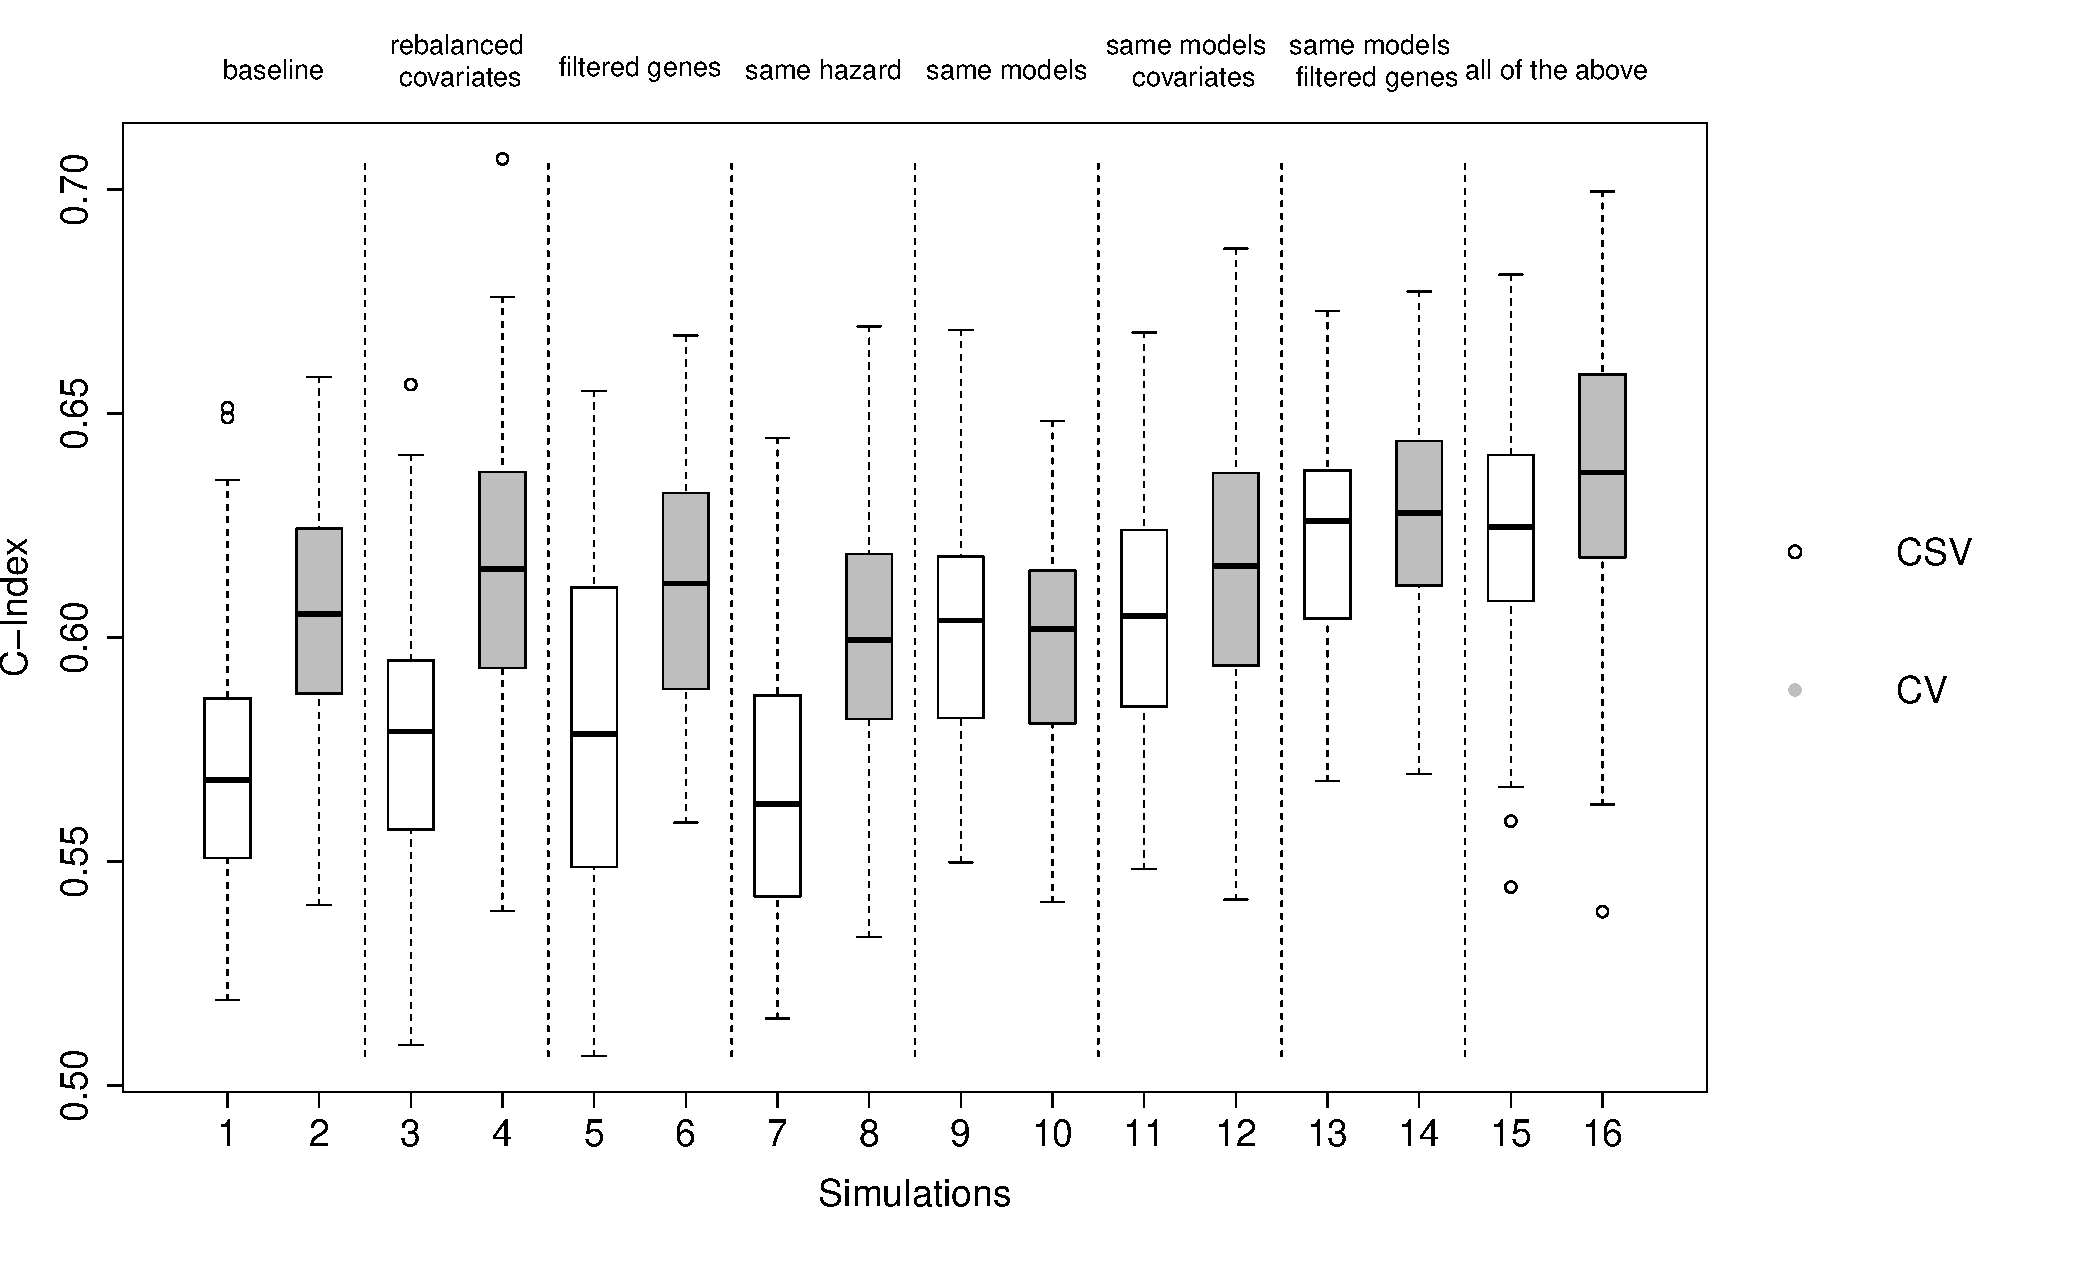
\includegraphics[width=16cm]{boxplot_breast_masomenos_allpanels.pdf}
   \end{figure}
   
  \begin{figure}[H]
		\centering            
        %\end{minipage}
        %\begin{minipage}[b]{1\textwidth}
        	\centerline{Breast Cancer / Ridge Regression}
            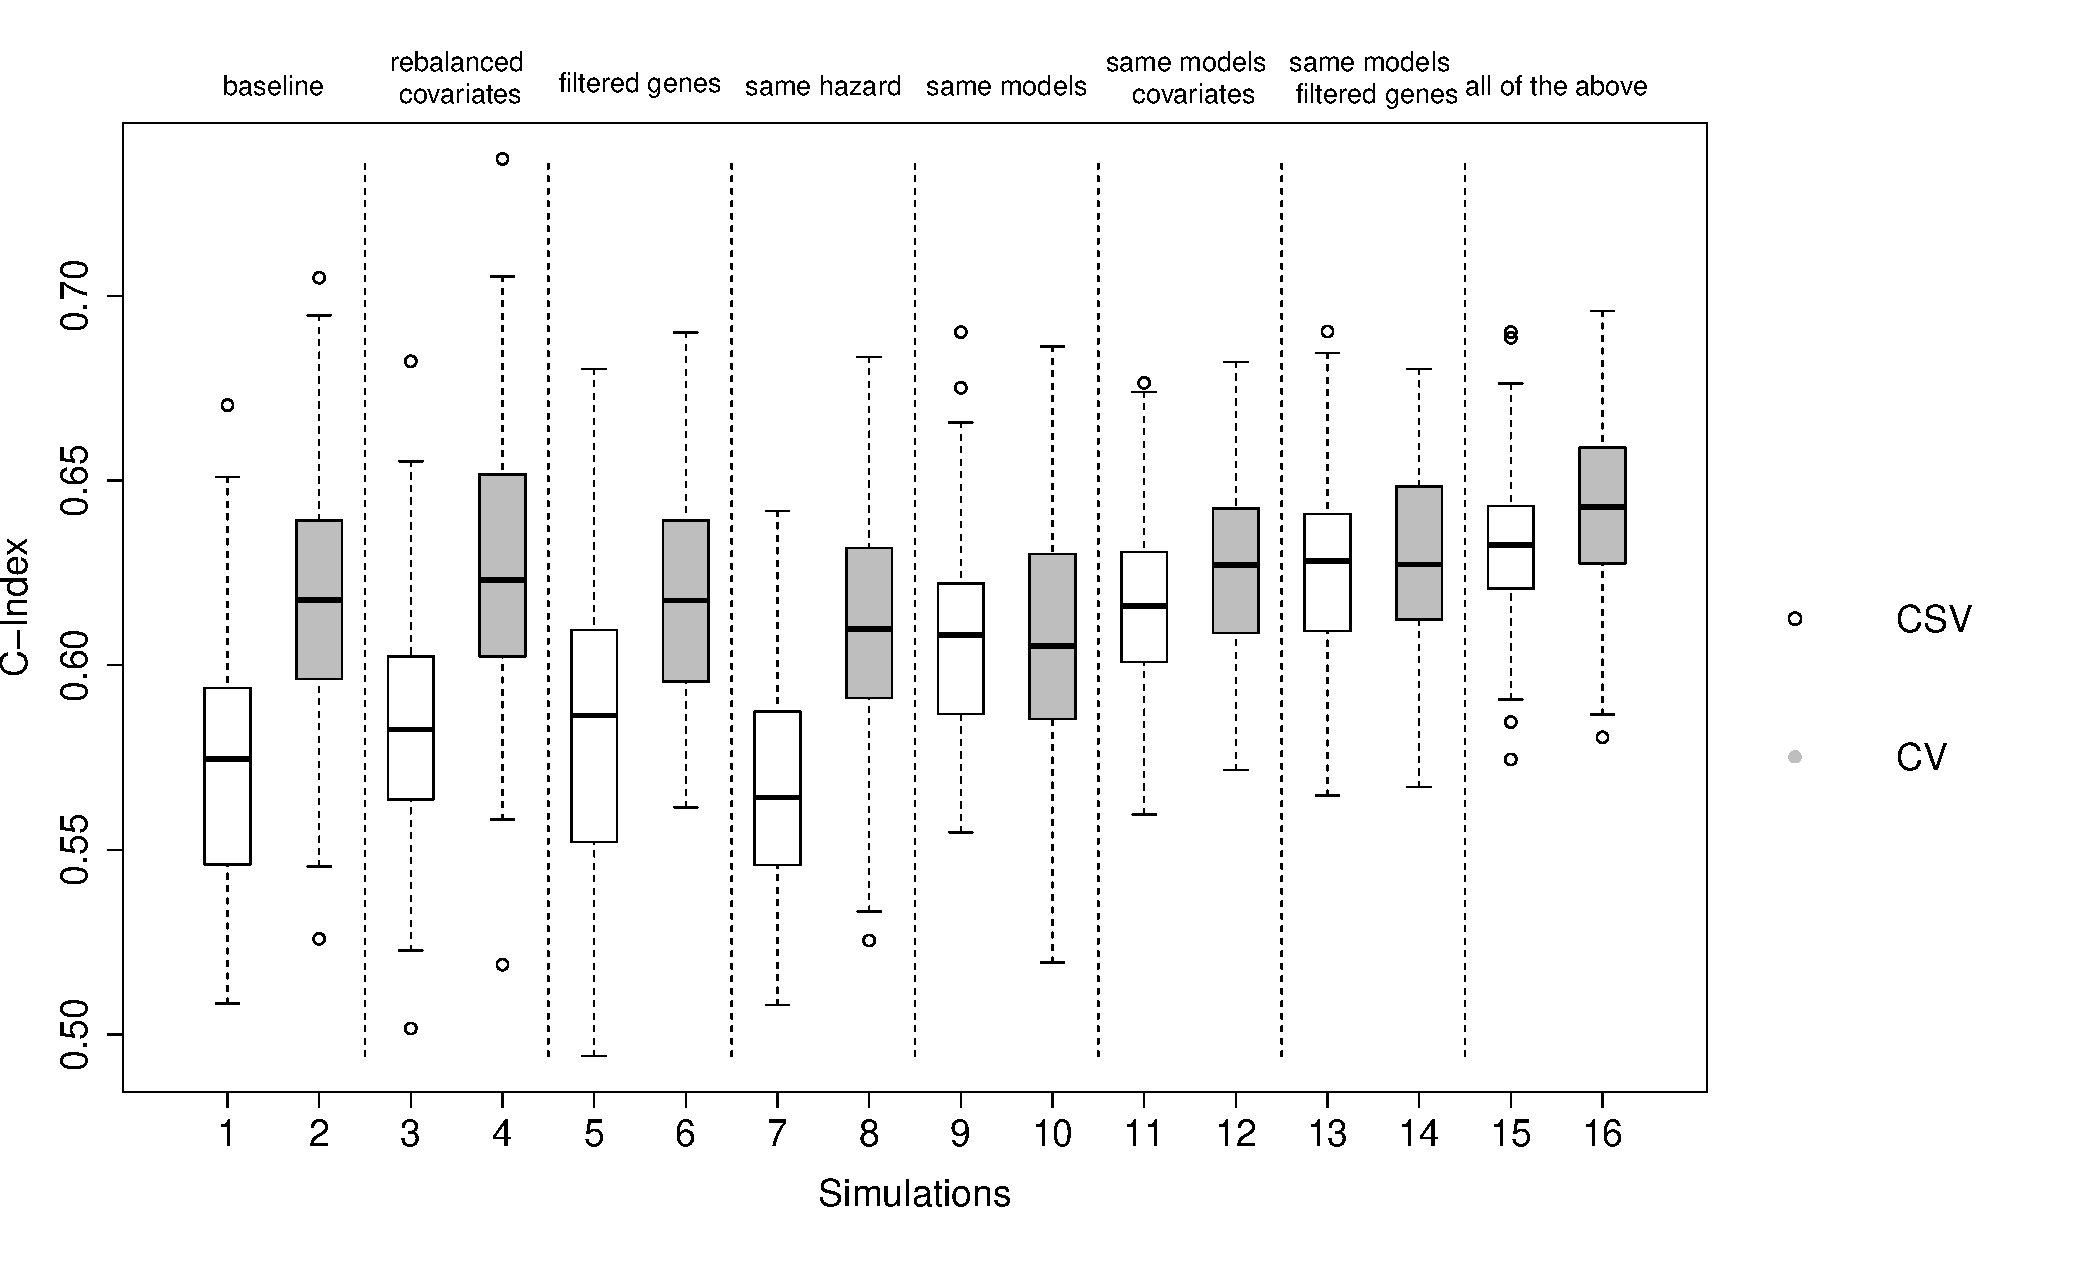
\includegraphics[width=16cm]{boxplot_breast_ridge_allpanels.pdf}
   \end{figure}
   
   \begin{figure}[H]
   		\centering            
        %\end{minipage}
        %\begin{minipage}[b]{1\textwidth}
      		\centerline{Ovarian Cancer / M\'{a}s-o-menos}
            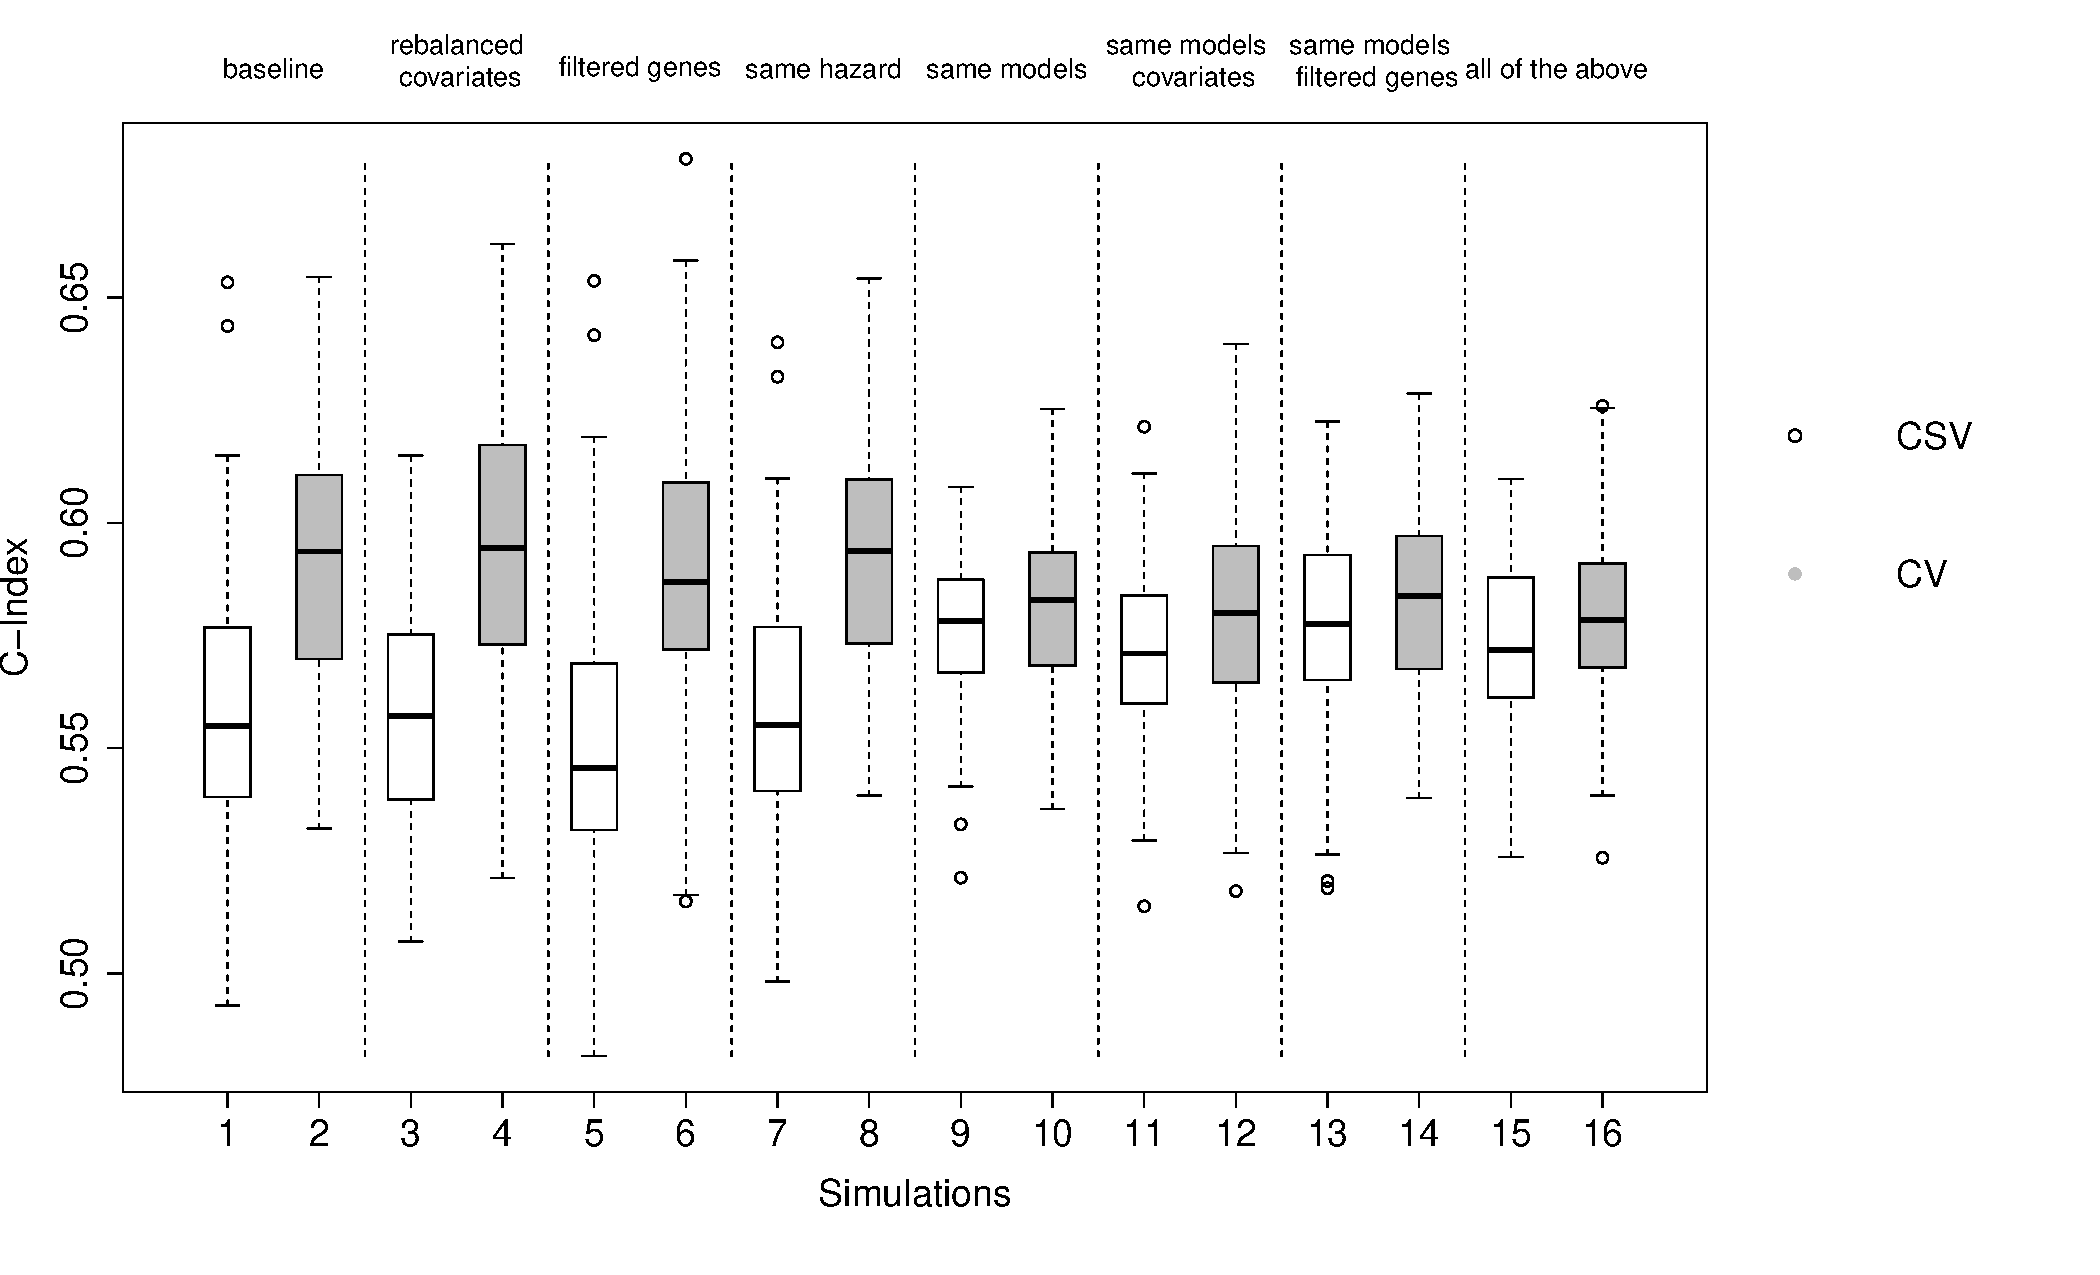
\includegraphics[width=16cm]{boxplot_ovarian_masomenos_allpanels.pdf}
         \caption{Simulation results comparing performances of cross validation and cross-study validation, in all three data / algorithm combinations, considering both single and multiple factors. Results for manipulating single sources in the other two dataset / algorithm combinations accord with the trends in Figure 2 and our conclusions in the main article. Altering multiple factors yields results that have a less clear interpretation. Panel names "baseline", "rebalanced covariates", "filtered genes", "same hazard" and "same models" are the same as Figure 2 in the main paper. "same models covariates" refers to using identical models while balancing covariates at the same time. "same models filtered genes" means filtering genes with high Integrative Correlation, then fit the same true models. In "all of the above", all three heterogeneity sources were equalized. A gap is reintroduced in between CV and CSV in this panel compared to using only identical models, which is more related to the rebalancing of covariates than filtering genes.}
         \label{boxplots}
    \end{figure}         
        %\end{minipage}


\newpage
\section{Availability of Covariates in Breast Cancer Data}
\begin{table}[H]
  \centering
    \begin{tabular}{rrrrrrrrrrr}
    \toprule
    name  &       & \multicolumn{1}{l}{CAL} & \multicolumn{1}{l}{MNZ} & \multicolumn{1}{l}{MSK} & \multicolumn{1}{l}{TAM1} & \multicolumn{1}{l}{TAM2} & \multicolumn{1}{l}{TRB} & \multicolumn{1}{l}{UNT} & \multicolumn{1}{l}{VDX} & \multicolumn{1}{l}{Overall} \\
    \midrule
    ER+   &       & 75    & 162   & 57    & 507   & 325   & 134   & 86    & 209   & 1555 \\
    \multicolumn{1}{c}{\multirow{3}[0]{*}{pgr  }} & availablity & 75    & /     & 57    & 65    & 321   & /     & 52    & /     & 570 \\
    \multicolumn{1}{c}{} & 0     & 17    & /     & 15    & 5     & 72    & /     & 1     & /     & 110 \\
    \multicolumn{1}{c}{} & 1     & 58    & /     & 42    & 60    & 249   & /     & 51    & /     & 460 \\
    \multicolumn{1}{c}{\multirow{3}[0]{*}{her2  }} & availablity & /     & /     & 49    & /     & 149   & /     & /     & /     & 198 \\
    \multicolumn{1}{c}{} & 0     & /     & /     & 0     & /     & 110   & /     & /     & /     & 110 \\
    \multicolumn{1}{c}{} & 1     & /     & /     & 49    & /     & 39    & /     & /     & /     & 88 \\
    \multicolumn{1}{c}{\multirow{3}[0]{*}{size}} & availablity & 74    & 162   & 57    & 341   & 164   & 134   & 86    & 209   & 1227 \\
    \multicolumn{1}{c}{} & 0     & 29    & 96    & 8     & 138   & 77    & 76    & 55    & 203   & 698 \\
    \multicolumn{1}{c}{} & 1     & 45    & 66    & 49    & 203   & 87    & 58    & 31    & 6     & 529 \\
    \multicolumn{1}{c}{\multirow{3}[0]{*}{node }} & availablity & 75    & 162   & 57    & 493   & 164   & 134   & 86    & 209   & 1380 \\
    \multicolumn{1}{c}{} & 0     & 32    & /   & 15    & 331   & 70    & /   & /    & /   & 1039 \\
    \multicolumn{1}{c}{} & 1     & 43    & /     & 42    & 162   & 94    & /     & /     & /     & 341 \\
    \multicolumn{1}{c}{\multirow{3}[0]{*}{age }} & availablity & 74    & 162   & 57    & 371   & 324   & 134   & 86    & 209   & 1417 \\
    \multicolumn{1}{c}{} & 0     & 31    & 38    & 22    & 32    & 59    & 95    & 32    & 90    & 399 \\
    \multicolumn{1}{c}{} & 1     & 43    & 124   & 35    & 339   & 265   & 39    & 54    & 119   & 1018 \\
    \multicolumn{1}{c}{\multirow{4}[0]{*}{grade}} & availablity & 74    & 162   & /     & 346   & 286   & 132   & 72    & 142   & 1214 \\
    \multicolumn{1}{c}{} & 1     & 5     & 27    & /     & 77    & 56    & 29    & 29    & 4     & 227 \\
    \multicolumn{1}{c}{} & 2     & 26    & 119   & /     & 202   & 134   & 68    & 31    & 36    & 616 \\
    \multicolumn{1}{c}{} & 3     & 43    & 16    & /     & 67    & 96    & 35    & 12    & 102   & 371 \\

  \bottomrule
  \end{tabular}
  \caption{Availability of covariates in 8 breast cancer data sets. The table reports the number of  patients left in the datasets after initial cleaning. Patient age and tumor size are dichotomized. size = tumor size, age = age of patients at diagnosis, node = nodal status,  grade = historical grade. Datasets acronyms are the same as Table 1 in the main article.}
  \label{table-cov}
\end{table}


\newpage
\section{Hazard Ratio of Covariates}  
  
  \begin{table}[H]
  \centering
    \begin{tabular}{llrr}
    \toprule
    Cov & HR & Confidence Interval & \#datasets\\
    \midrule
    Size  & 1.96  & [1.46 , 2.62] & 7 \\
    Age   & 1.2   & [0.86 , 1.65] & 6 \\
%    Nodal Status & 2.04  & [1.40 , 2.97] & 3 \\
    Histological Grade & 1.65  & [1.24 , 2.19] & 7 \\
    \bottomrule
    \end{tabular}
    \caption{\textbf{Synthesized hazard ratios of all covariates in the breast cancer datasets.}
       The three-level histological grade is dichotomized for the calculation of HR, by combining the low and intermediate levels as 0, and treating the high level as 1. Row labels: Cov = covariate names, HR =
      hazard ratio synthesized across all base datasets by
      fixed-effects meta-analysis. Interval =
      95\% Confidence Interval, \#datasets = Number of studies available for
      hazard ratio. Tumor size and
      histological grade, but not age dichotomized at 50 years, are significantly associated with
      disease and metastasis-free survival. }
  \label{HR-table}
\end{table}

  \begin{table}[H]
  \centering
    \begin{tabular}{llrr}
    \toprule
    Cov & HR & Confidence Interval & \#datasets\\
    \midrule
    Age  &  1.84 & [1.51 , 2.24] & 5 \\
    Debulking  & 1.48   & [1.23 , 1.78] & 5 \\
    %Histological Grade & 1.52  & [1.20 , 1.93] & 5 \\
    %Cancer Stage & 3.38  & [1.90 , 6.01] & 4 \\
    \bottomrule
    \end{tabular}
    \caption{\textbf{Synthesized hazard ratios of all covariates in the ovarian cancer datasets.}
      Row labels: Cov = covariate names, HR =
      hazard ratio synthesized across all datasets by
      fixed-effects meta-analysis. Interval =
      95\% Confidence Interval, \#datasets = Number of studies available for
      hazard ratio. All factors are significantly associated with
      survival. }
  \label{HR-table-ovarian}
\end{table}


\newpage
\section{Forest Plots of Hazard Ratio of the Covariates}
\begin{figure}[H]
      \centering
      \centerline{Breast Cancer Clinical Covariates}
        \begin{minipage}[b]{0.5\textwidth}
            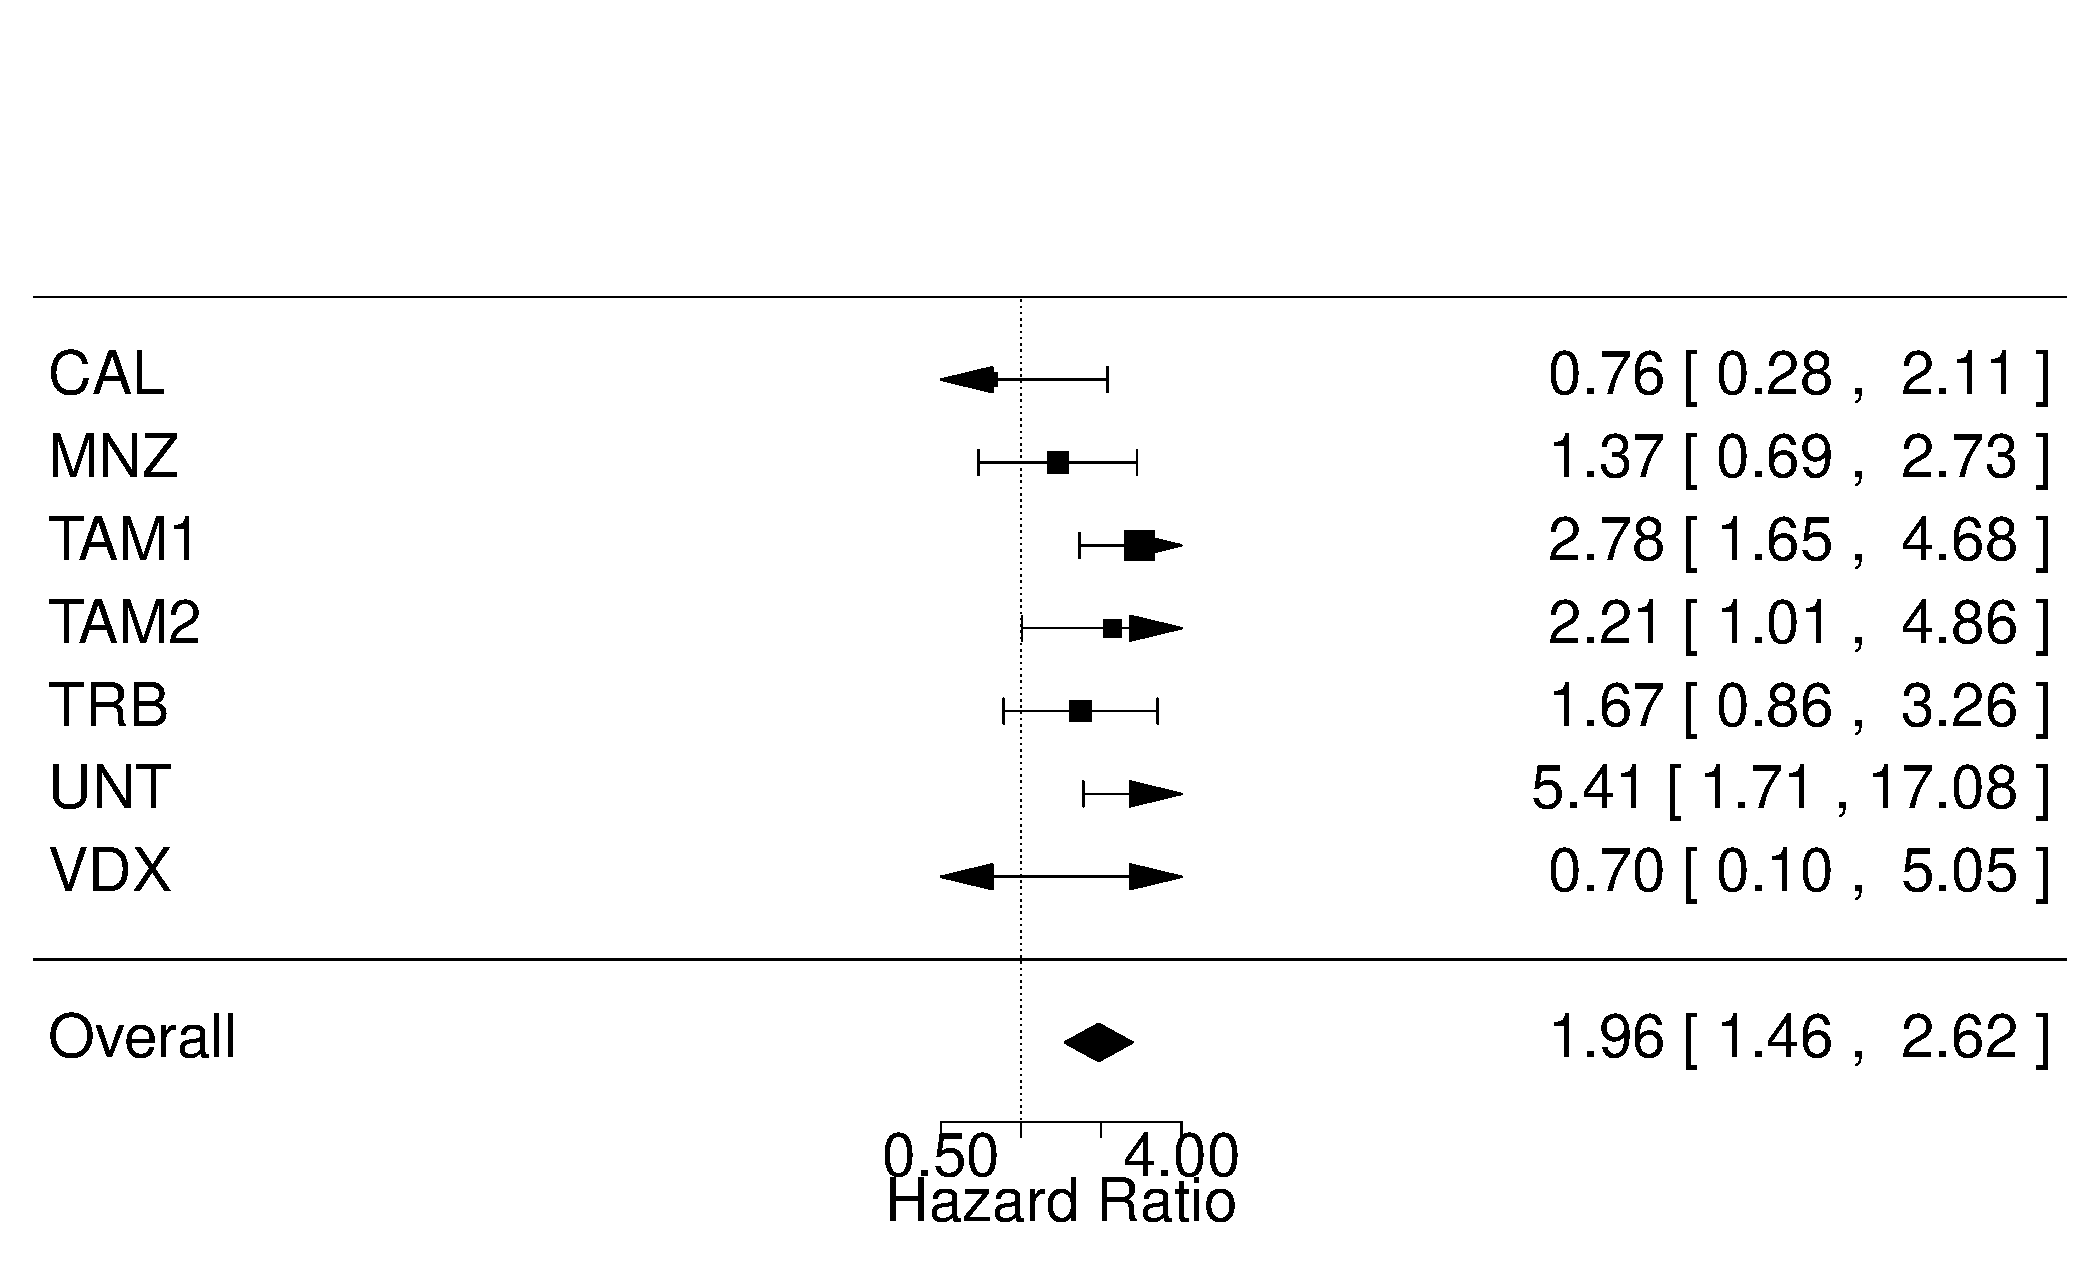
\includegraphics[width=8.8cm]{forest_size.pdf}
            \centerline{(a) Tumor Size}
        \end{minipage}%
        \begin{minipage}[b]{0.5\textwidth}
            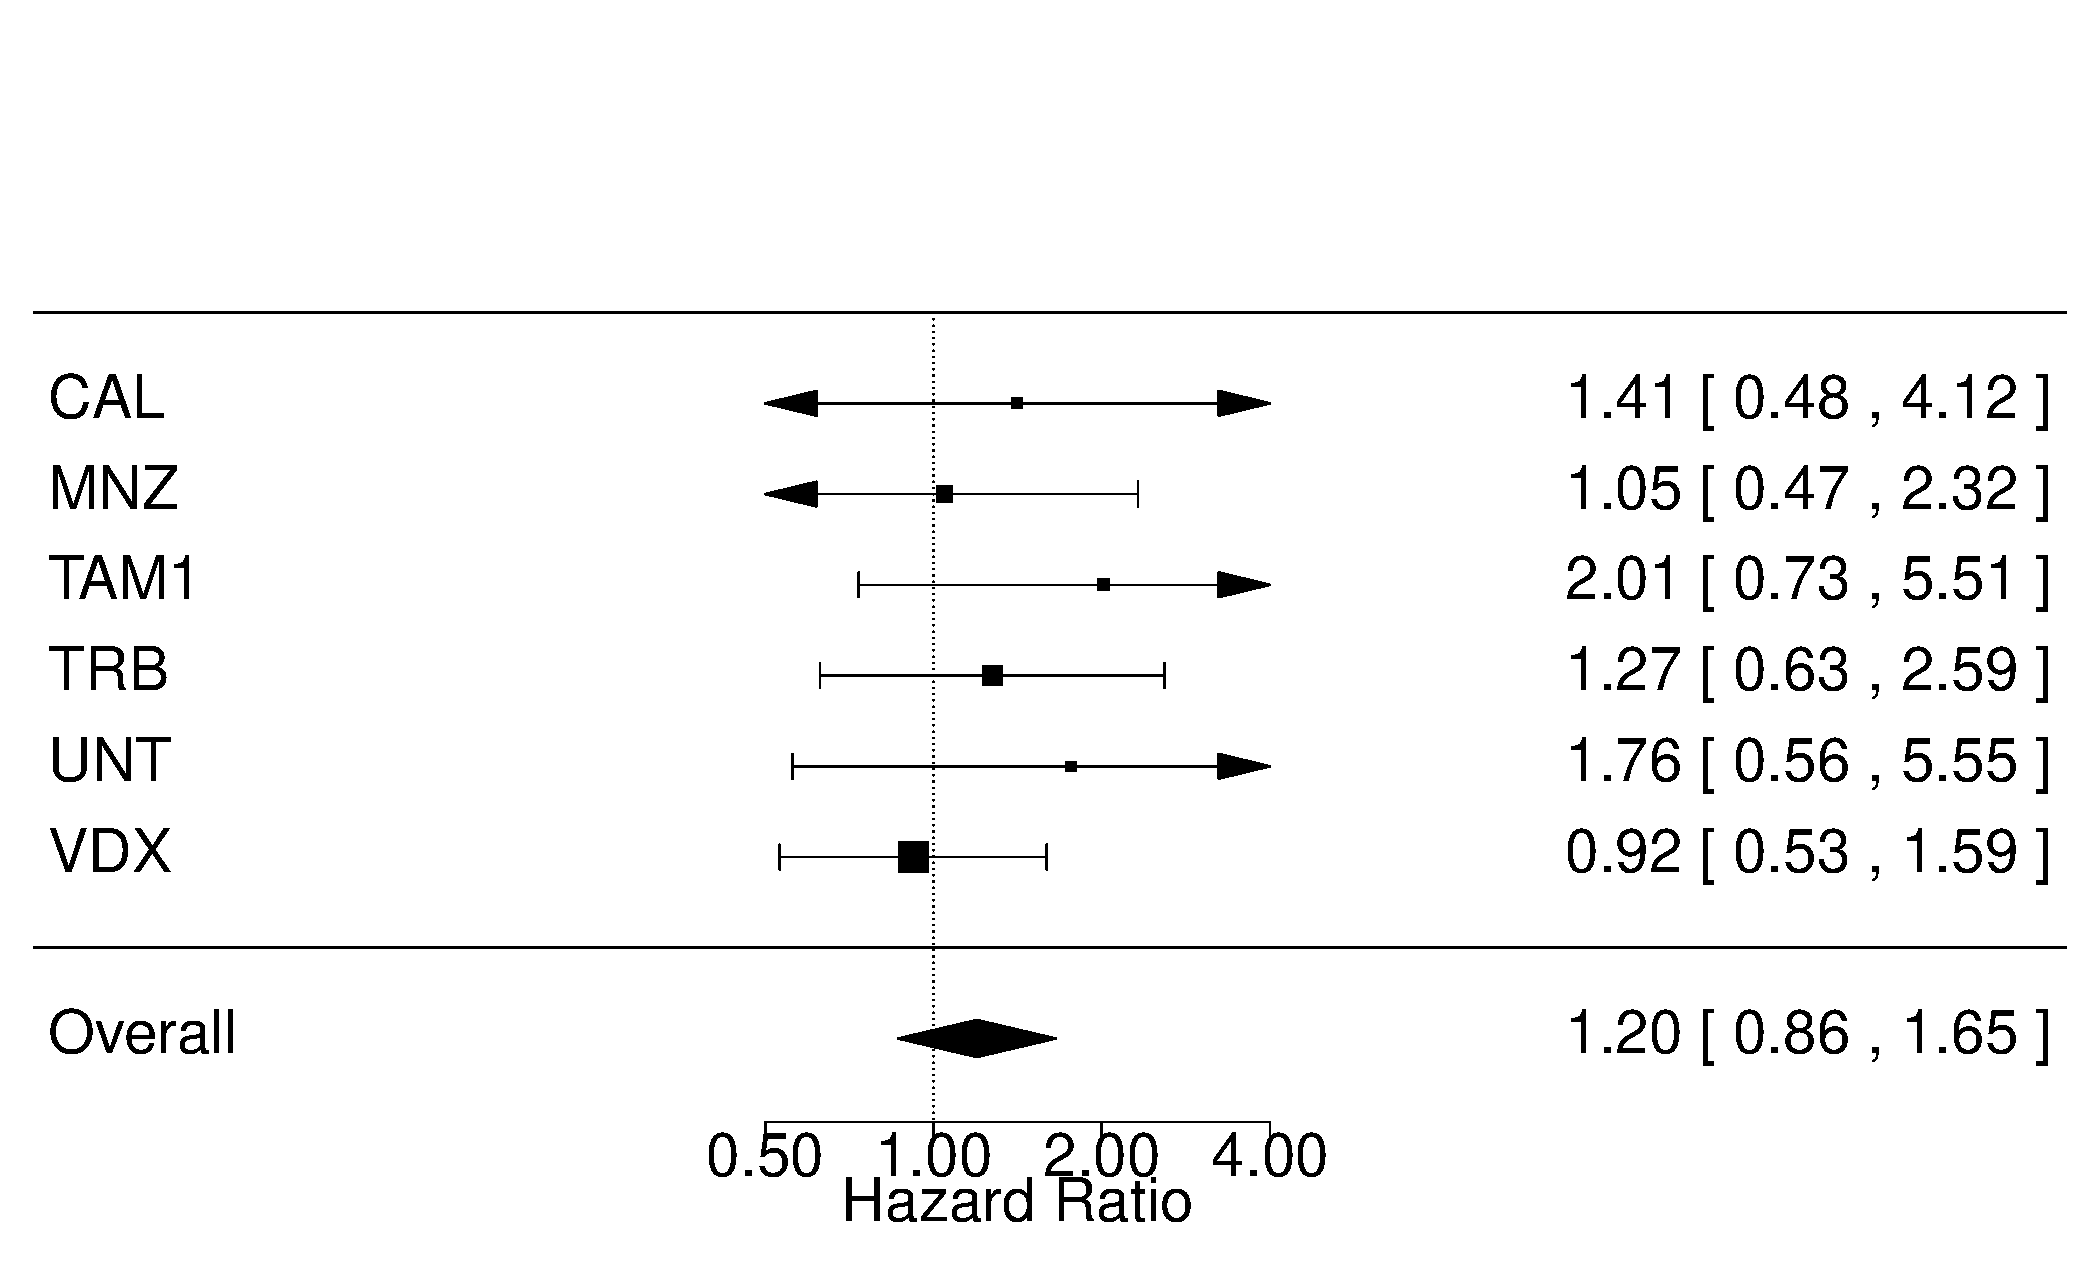
\includegraphics[width=8.8cm]{forest_age.pdf}
             \centerline{(b) Age}
        \end{minipage}
        %\begin{minipage}[b]{0.5\textwidth}
        %    \includegraphics[width=7cm]{forestplots-NEW-node.pdf}
        %    \centerline{(c) Nodal Status}
        %\end{minipage}%
        \begin{minipage}[b]{0.5\textwidth}
            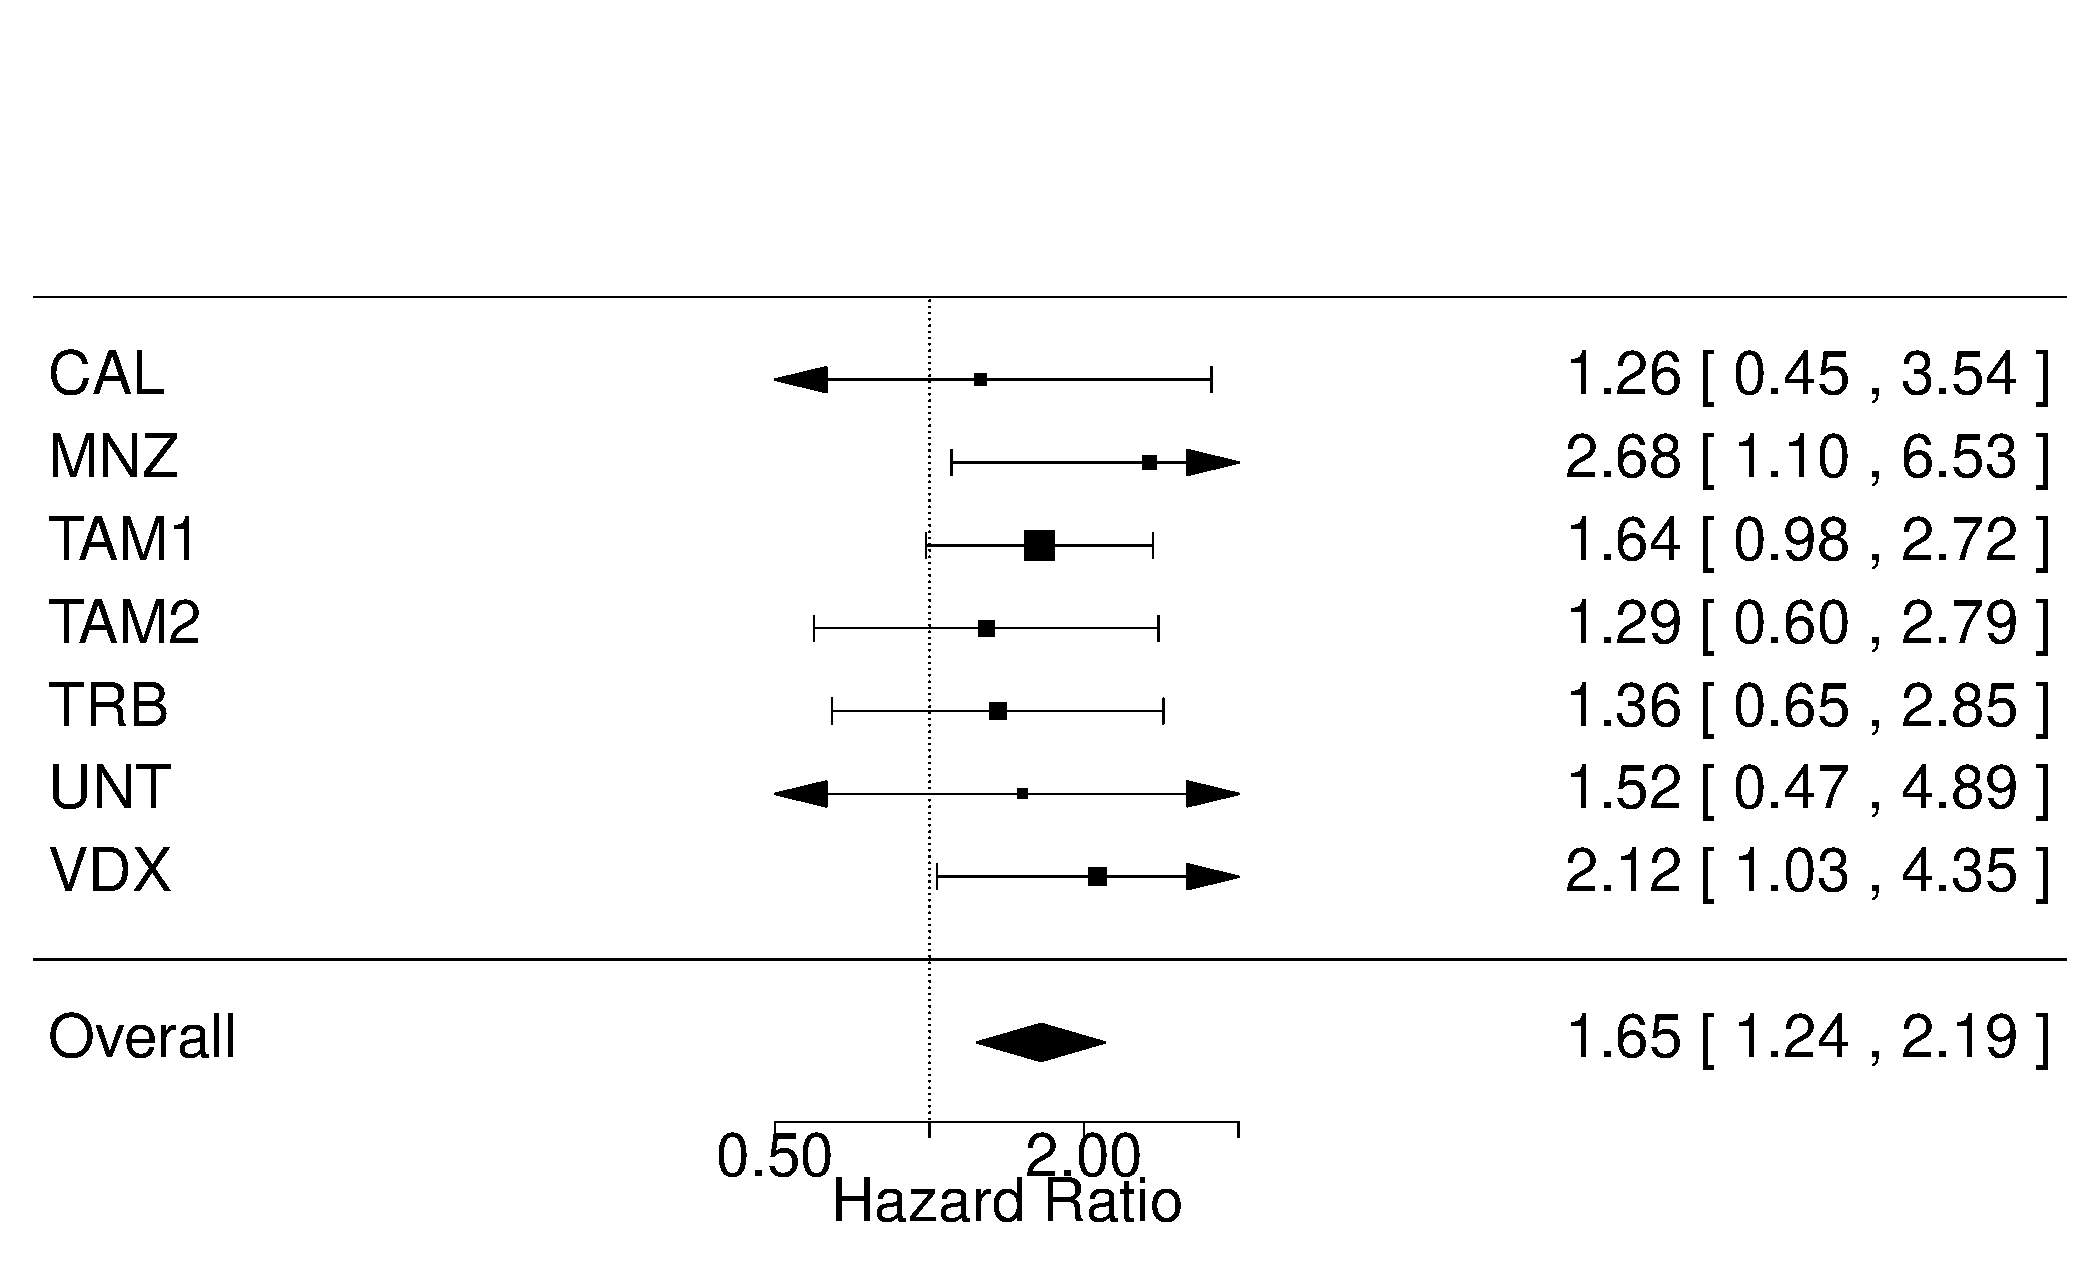
\includegraphics[width=8.8cm]{forest_grade.pdf}
            \centerline{(c) Histological Grade}
        \end{minipage}
    \label{forest-plots}
  \end{figure}
  
  \begin{figure}[H]
      \centering
      \centerline{Ovarian Cancer Clinical Covariates}
        \begin{minipage}[b]{0.5\textwidth}
            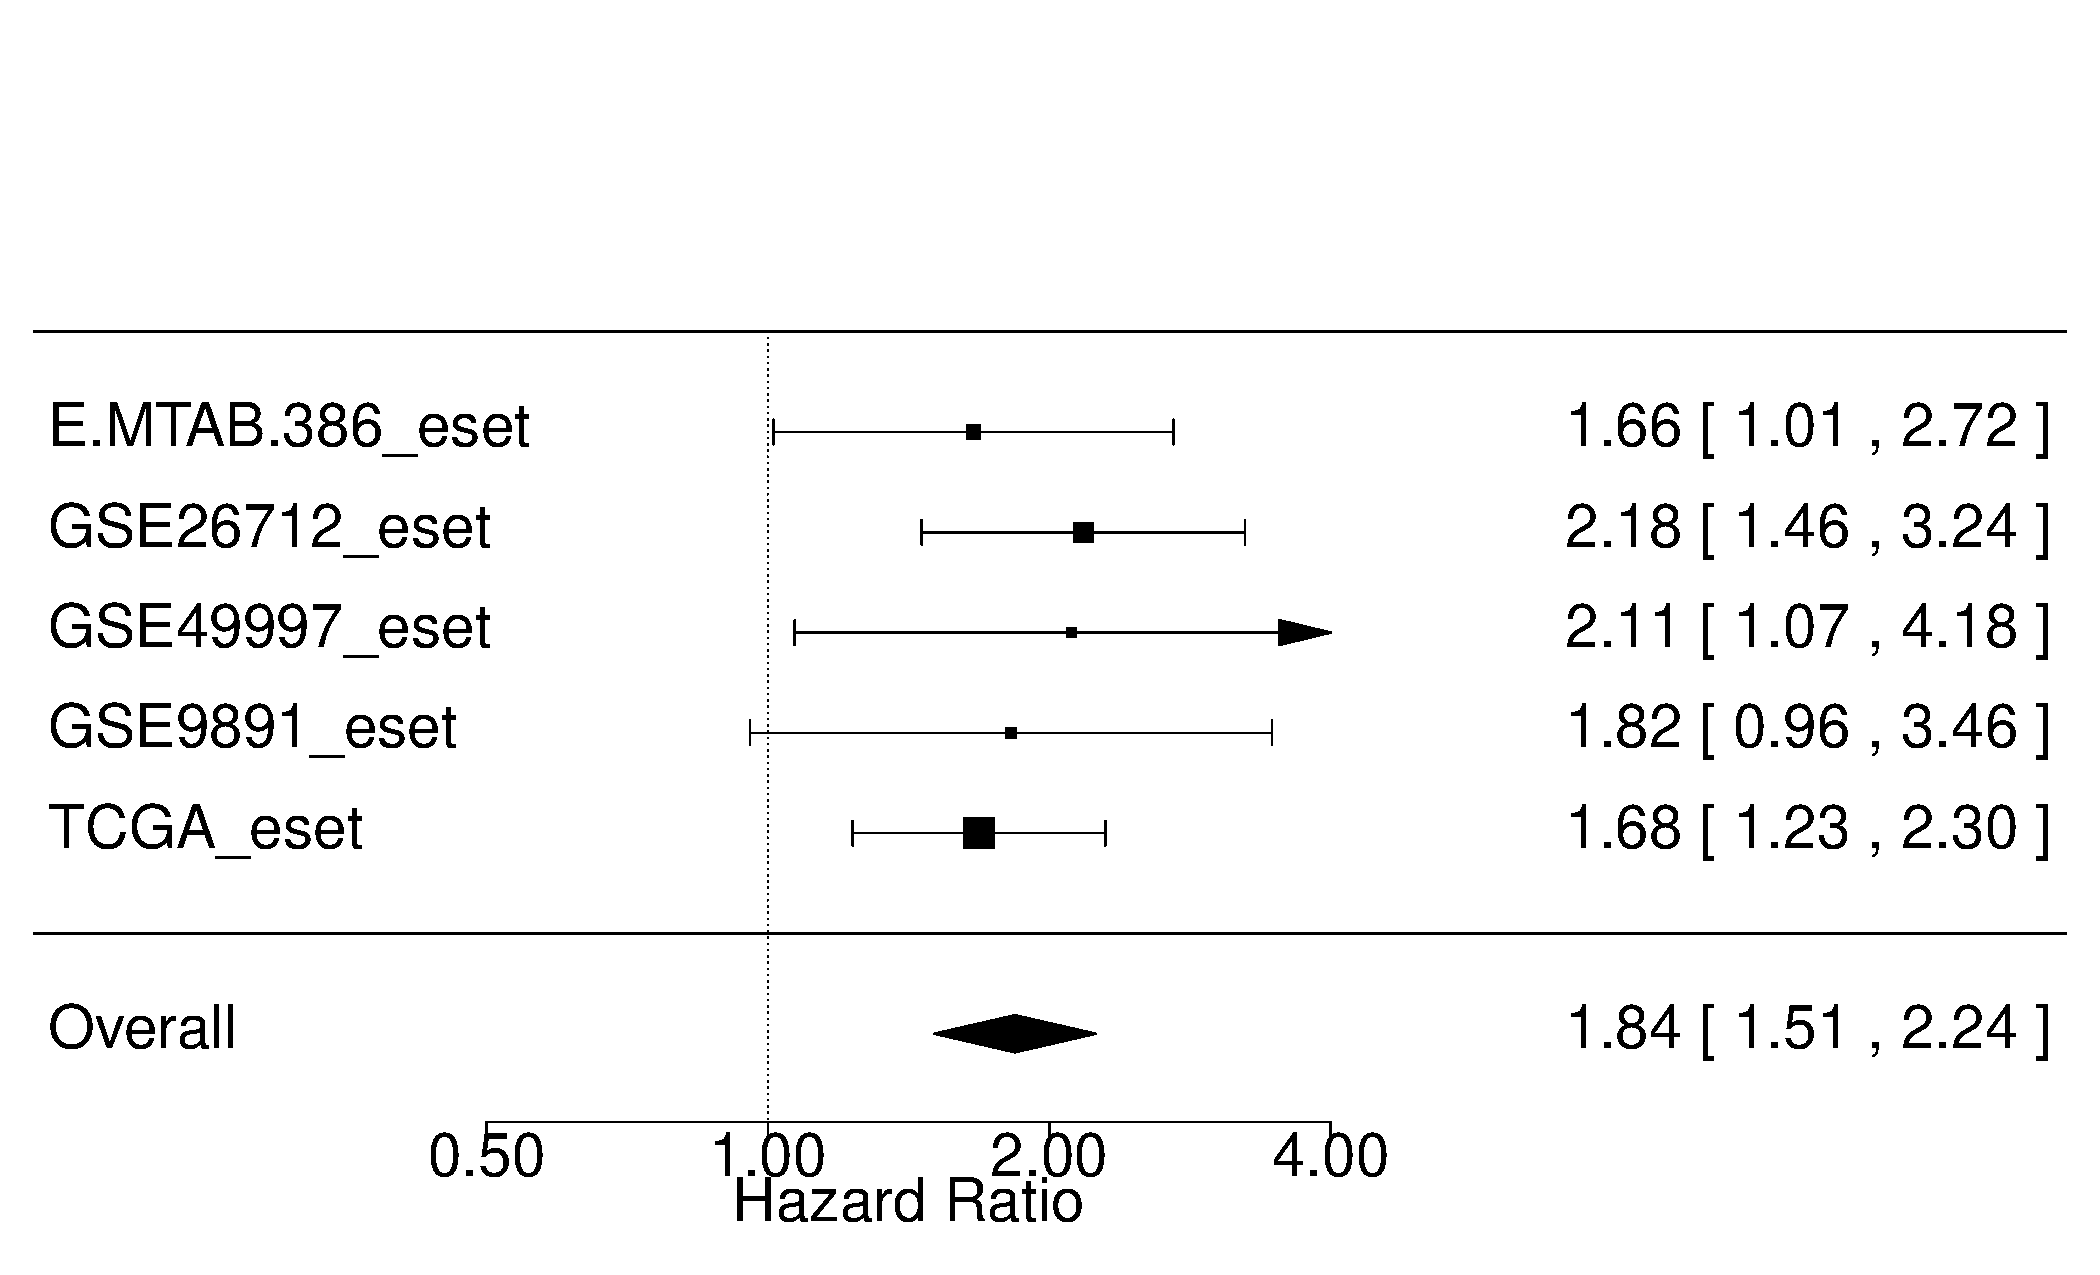
\includegraphics[width=8.8cm]{forest_ovarian_age.pdf}
            \centerline{(a) Age}
        \end{minipage}%
        \begin{minipage}[b]{0.5\textwidth}
            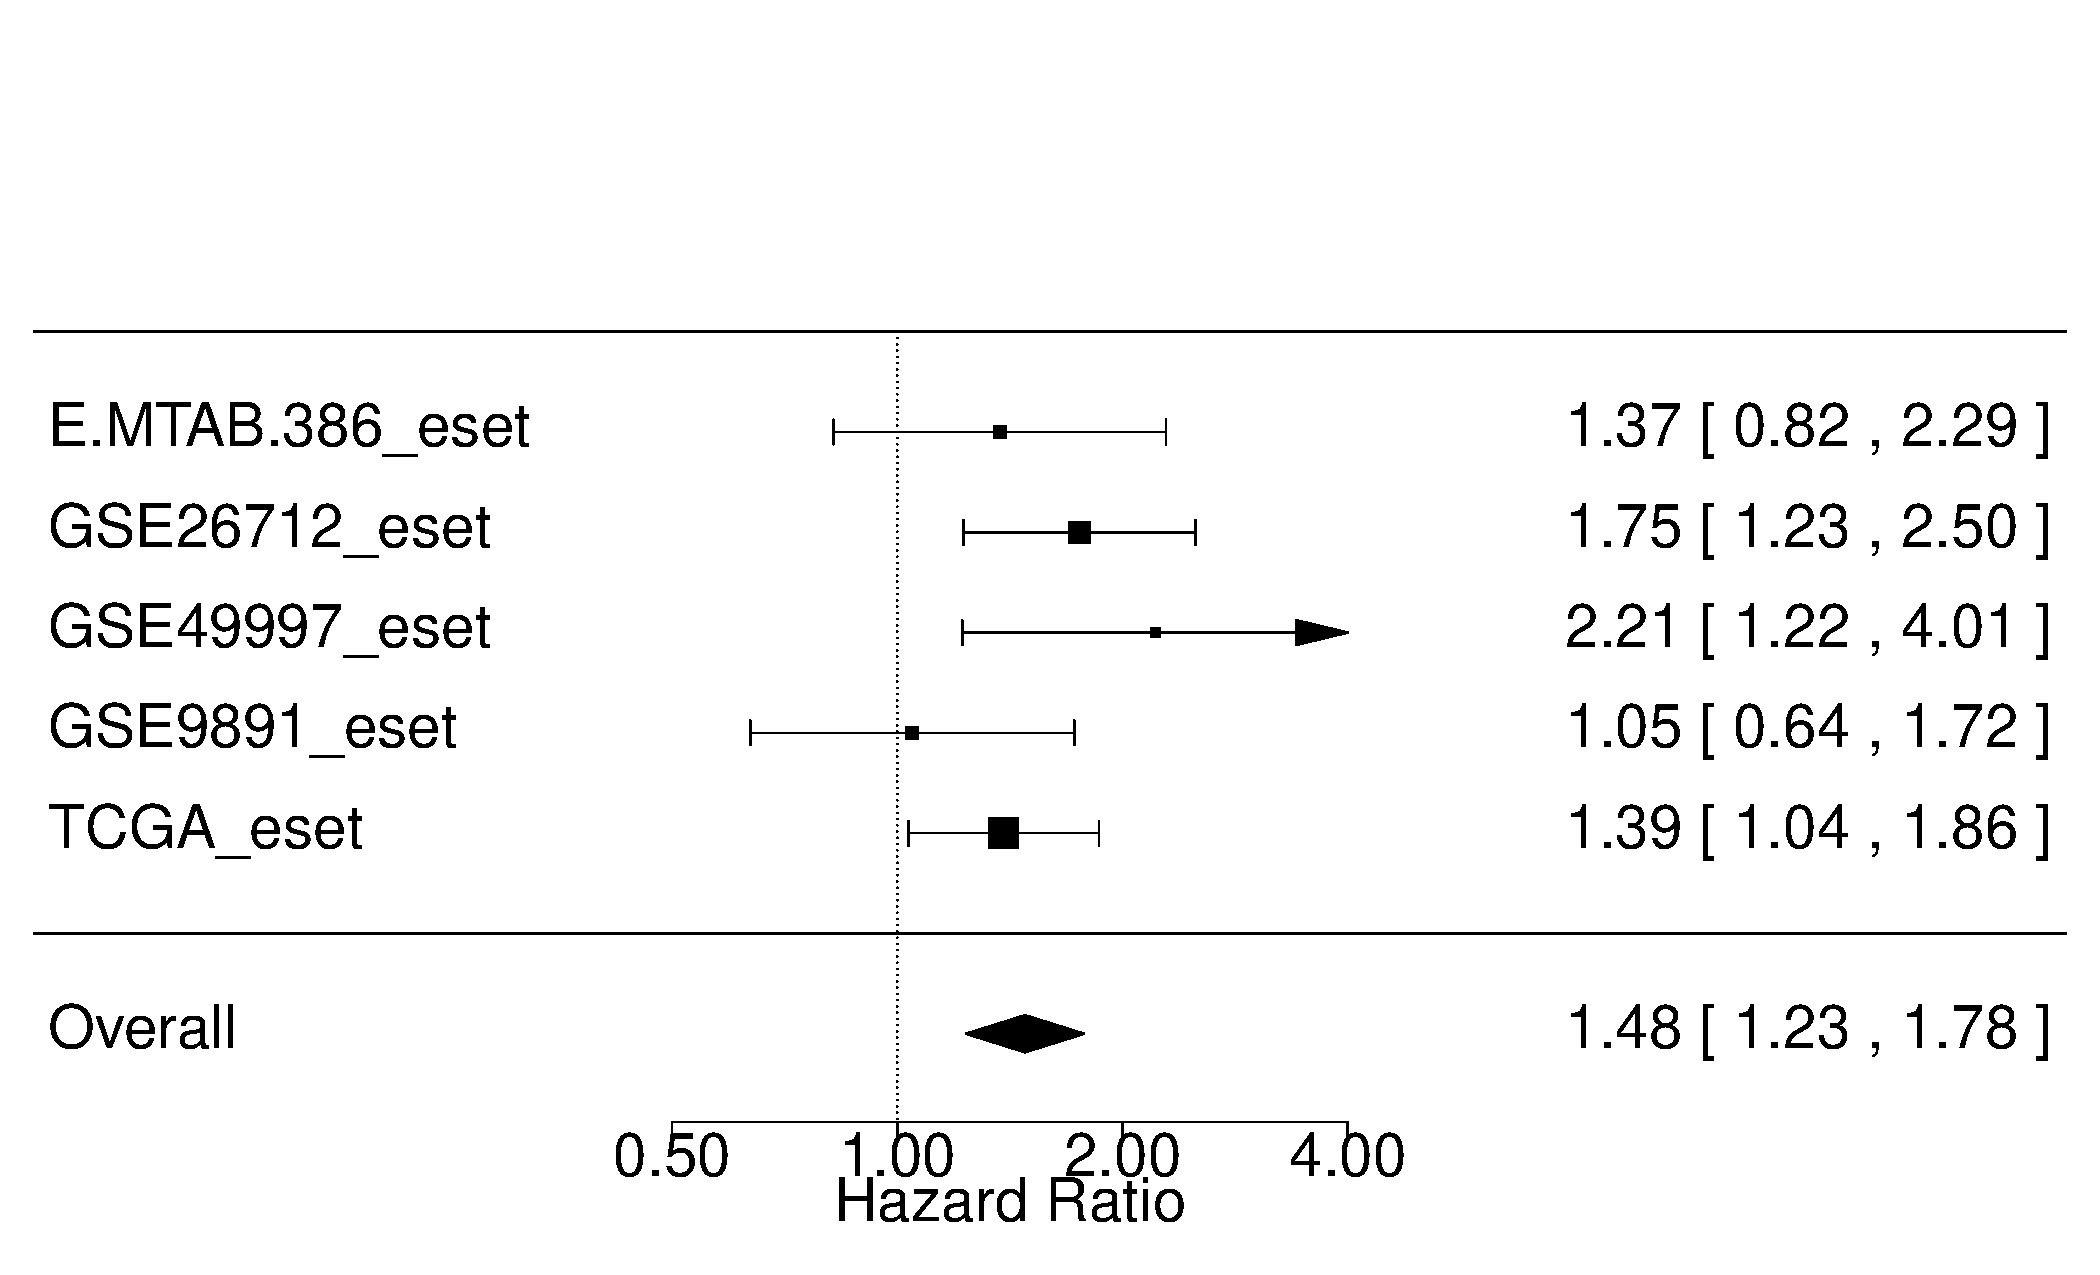
\includegraphics[width=8.8cm]{forest_ovarian_debulk.pdf}
             \centerline{(b) Debulking}
        \end{minipage}
%        \begin{minipage}[b]{0.5\textwidth}
%            \includegraphics[width=7cm]{forestplotOvarian-002-3.pdf}
%            \centerline{(c) Grade}
%        \end{minipage}%
%        \begin{minipage}[b]{0.5\textwidth}
%            \includegraphics[width=7cm]{forestplotOvarian-002-4.pdf}
%            \centerline{(d) Stage}
%        \end{minipage}
    \caption{Forest plots of hazard ratios to illustrate the relative strength of covariate impact in the studies. For breast cancer, at a certain level of confidence, the impacts of all these covariates significantly differ from no effect on the corresponding survival time, based on the deviance of overall confidence interval from the null hypothesis. %In panel(c) we only show studies in which we balance the prevalence of covariates. In the other studies, observations have only one level of nodal status making it impossible to balance. 
    For ovarian cancer, both factors significantly associate with survival. To show that the covariates we consider are prognostic further explains our finding that the distribution of these variables do not influence the validation performance.}
%    \caption{Forest plots of hazard ratios for ovarian cancer clinical factors to illustrate the relative strength of covariate impact in the studies. %At certain level of confidence, the impacts of all these covariates significantly differ from no effect on the corresponding survival time, based on the deviance of overall confidence interval from the null hypothesis. In panel(c) we only show studies in which we balance the prevalence of covariates. In the other studies, observations have only one level of nodal status making it impossible to balance. To show that the covariates we consider are prognostic further explains our finding that the distribution of these variables do not influence the validation performance.
%    Aside from debulking, the rest three factors significantly associate with survival. The number of datasets these covariates are available are also listed in the same way as above.}
    \label{forest-plots-ovarian}
  \end{figure}

\newpage
\section{Cross-study validation matrices using M\'{a}s-o-menos on the original and simulated breast cancer datasets}

\begin{figure}[H]
    \centering
    \begin{minipage}[b]{0.5\linewidth}
    \centerline{(a) original}
    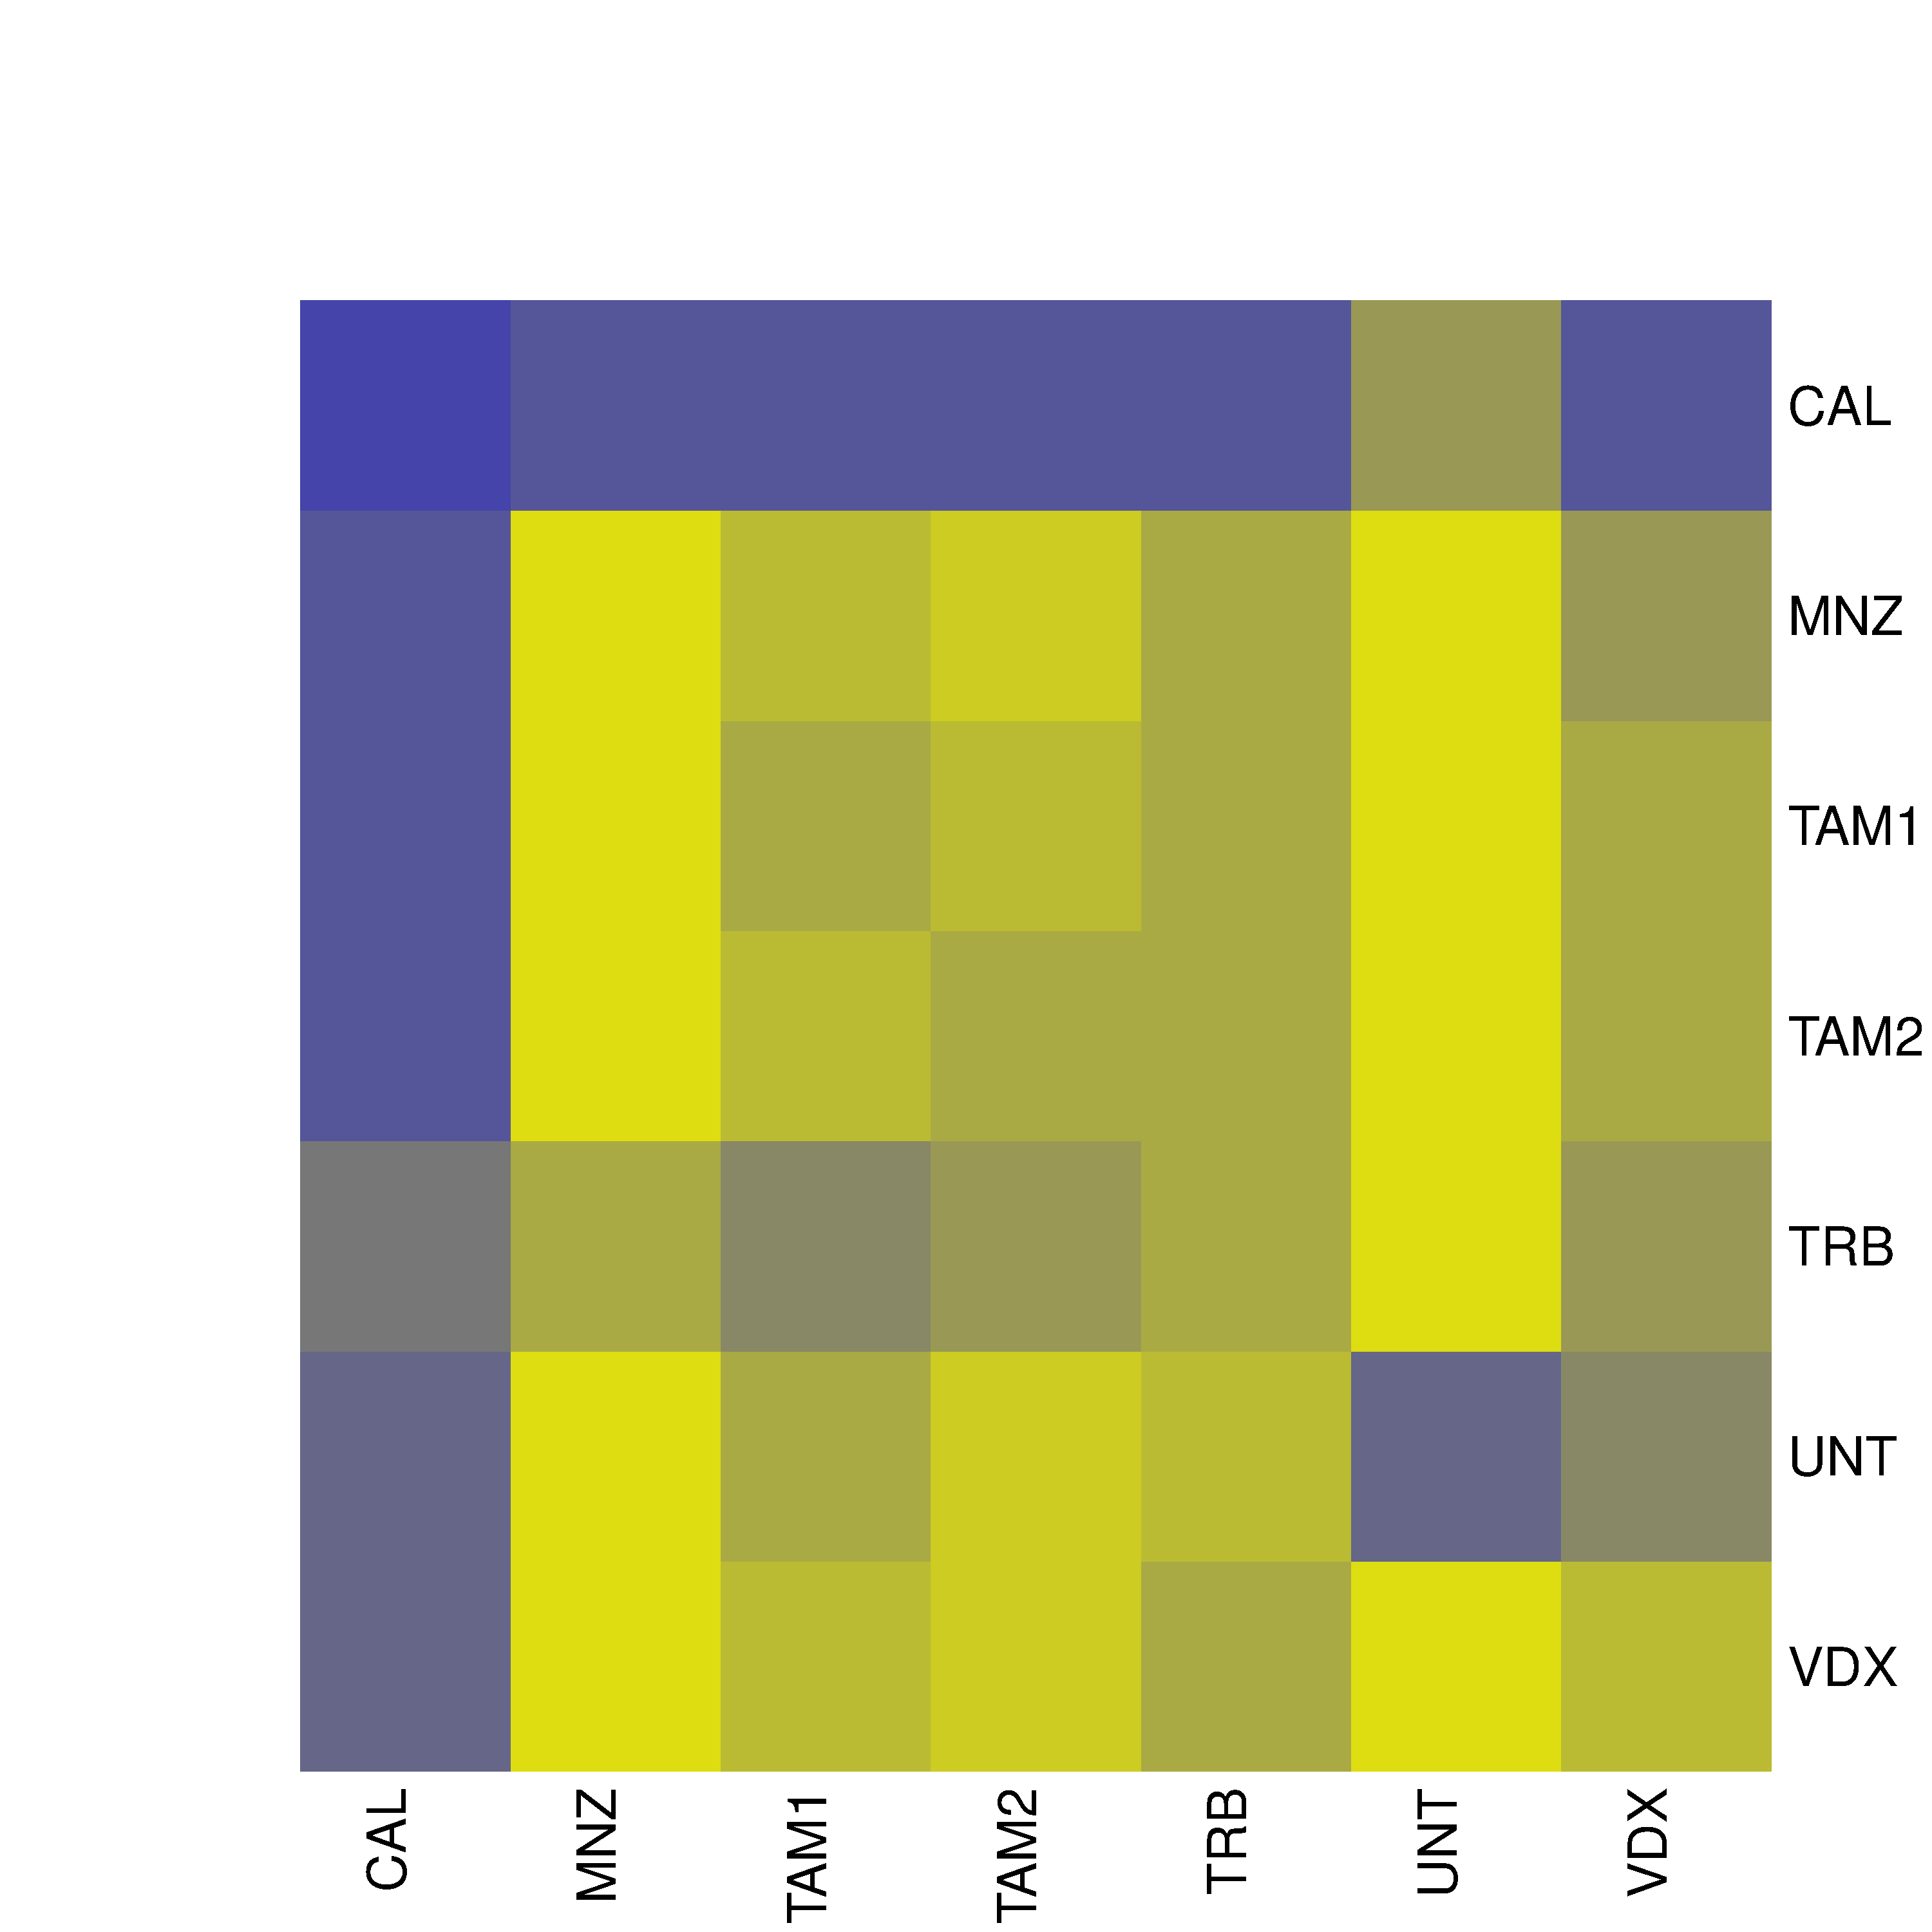
\includegraphics[width=7cm]{heatmap-a.pdf}
    \end{minipage}%
    \begin{minipage}[b]{0.5\linewidth}
    \centerline{(b) simulated}
    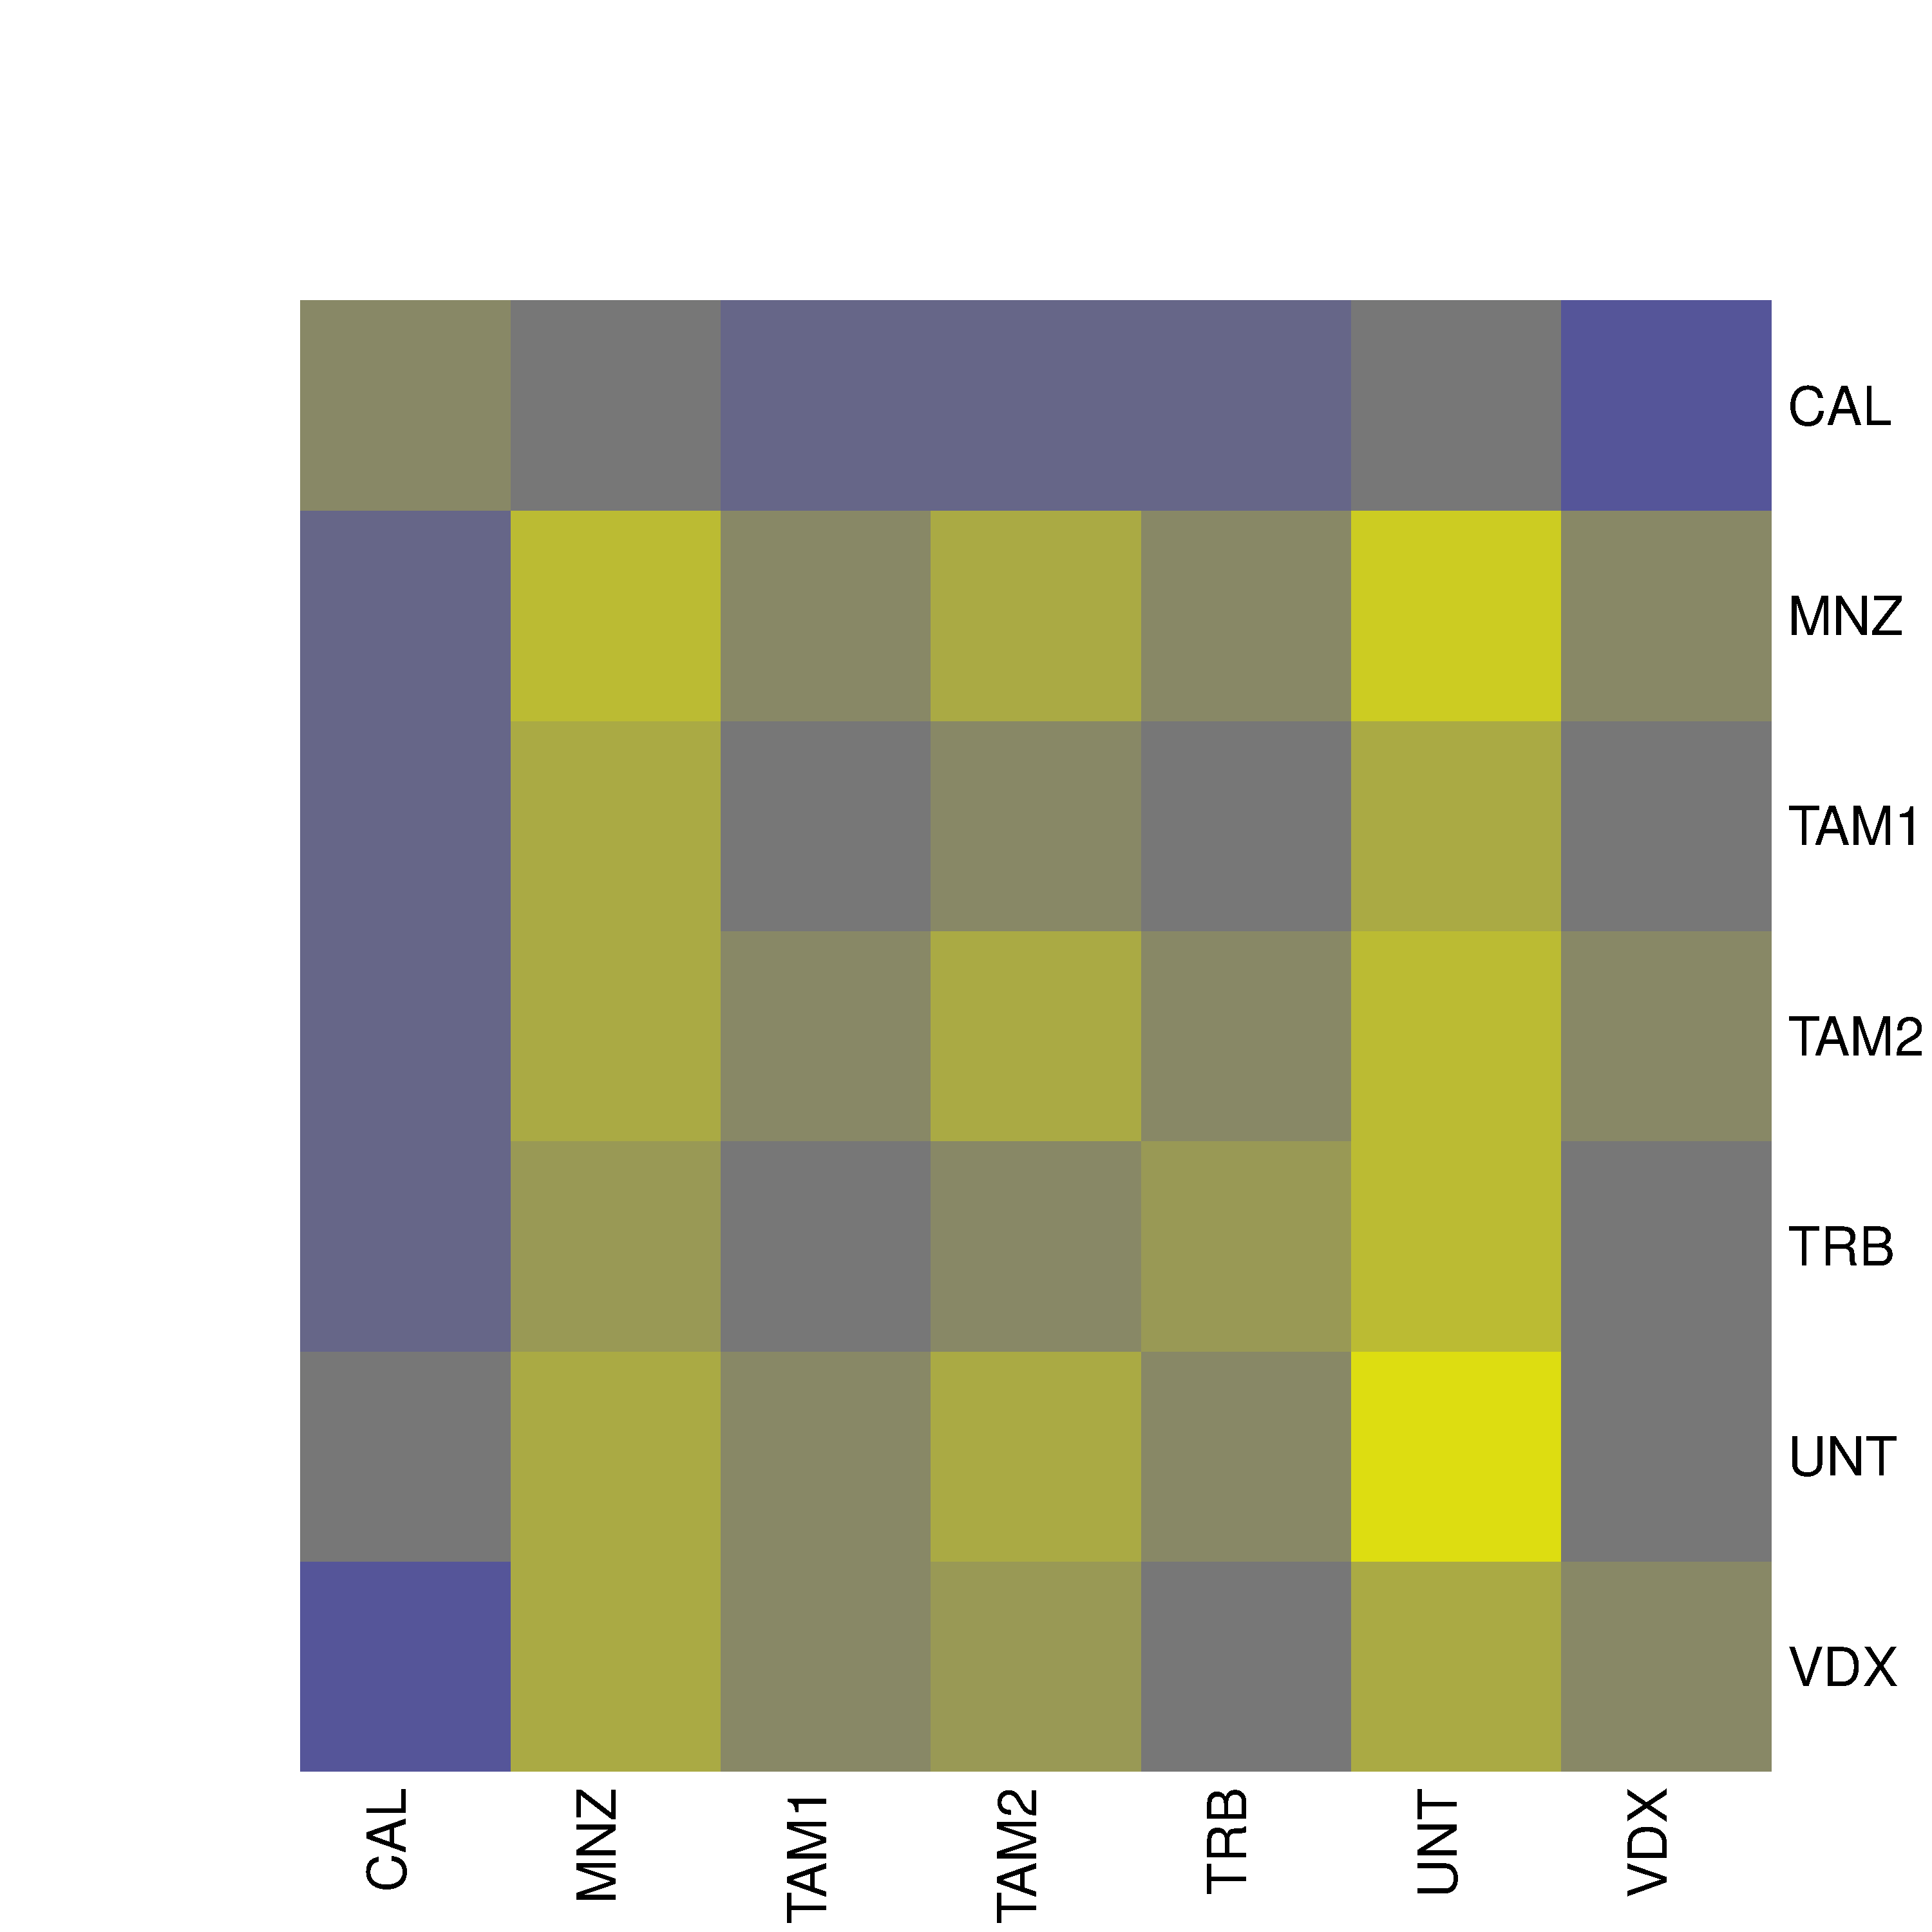
\includegraphics[width=7cm]{heatmap-b.pdf}
    \end{minipage}
    \caption{Cross-study validation matrices using
      M\'{a}s-o-menos algorithm on ER+ breast cancer data, showing
        comparability of simulated and experimental data for the
        purpose of discrimination of disease and metastasis-free survival. Panel (a)
      displays C-indices for training and validation on each pair of
      original datasets, with the diagonal showing results of
      4-fold CV. Panel (b) displays the equivalent heatmap, of the Z matrix
      averaged over 100 simulations, using
      simulated data generated by non-parametric bootstrap resampling
      of individuals and parametric simulation of censored time to event
      outcomes based on models estimated from the original base sets.
%      Panel (b) differs in that diagonal
%      elements show average C-index over pairs of independent datasets obtained by
%      resampling from the same study, rather than
%      cross-validation. 
      Within and across-study validation performance
      is similar between original and simulated data, with the
      exception of the outlier CAL
      dataset, which shows a larger difference in CV-CSV performances than the other datasets. Note that
      Bernau \textit{et al.} (2014) displayed one additional outlier set that was
      eliminated from this study due to unavailability
      of histological grade.}
    \label{heatmaps}
  \end{figure}
  

\newpage
\section{Bar-plots of covariate distributions before and after balancing}
\begin{figure}[H]
\centerline{Breast Cancer}
      \centering
        \begin{minipage}[b]{0.5\textwidth}
            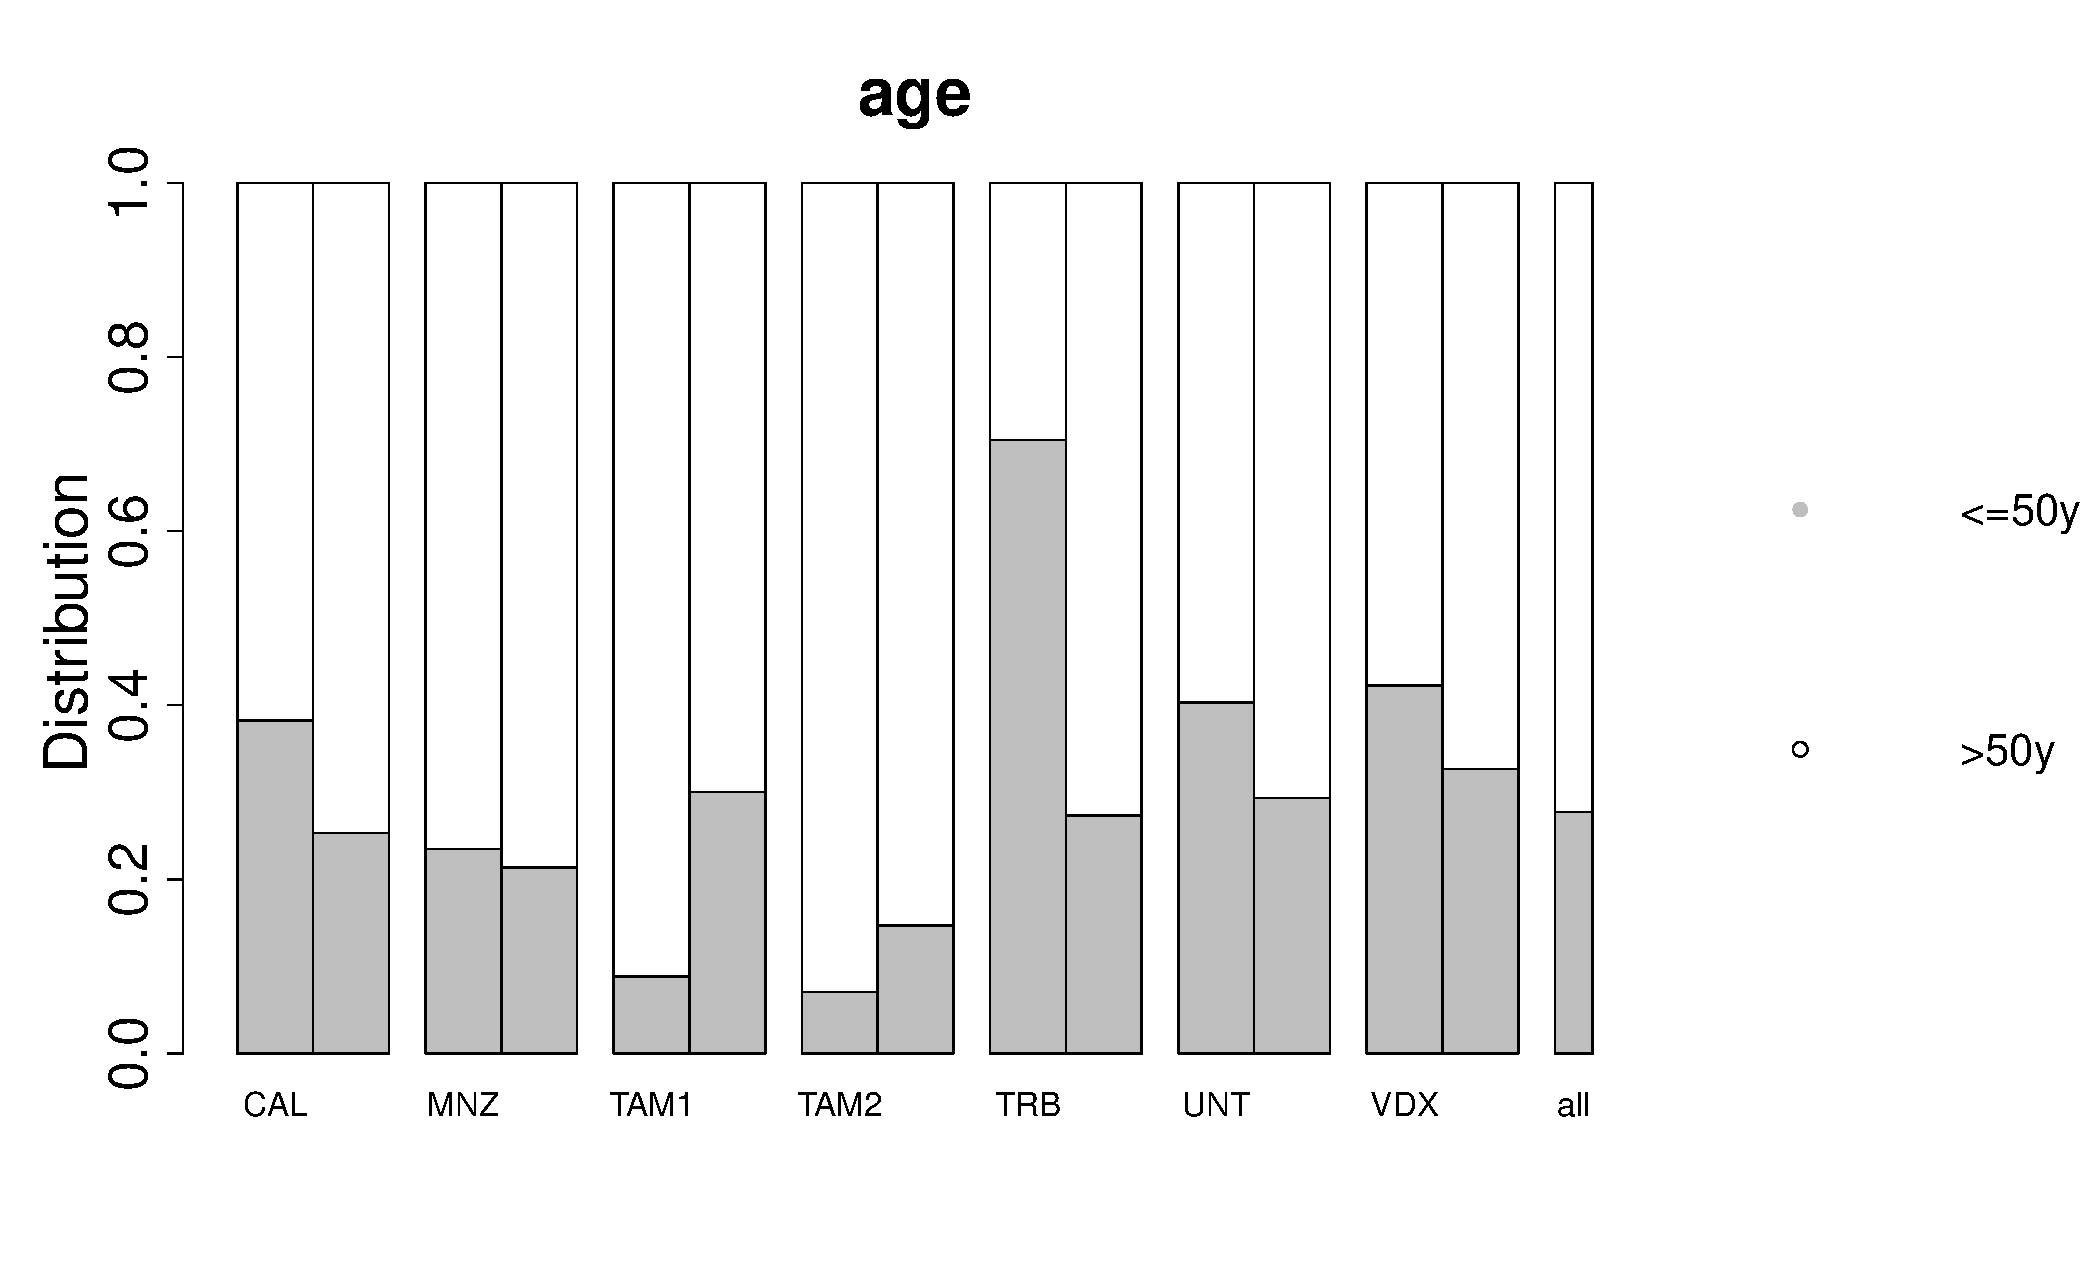
\includegraphics[width=8.5cm]{barplot_age.pdf}
        \end{minipage}%
        \begin{minipage}[b]{0.5\textwidth}
            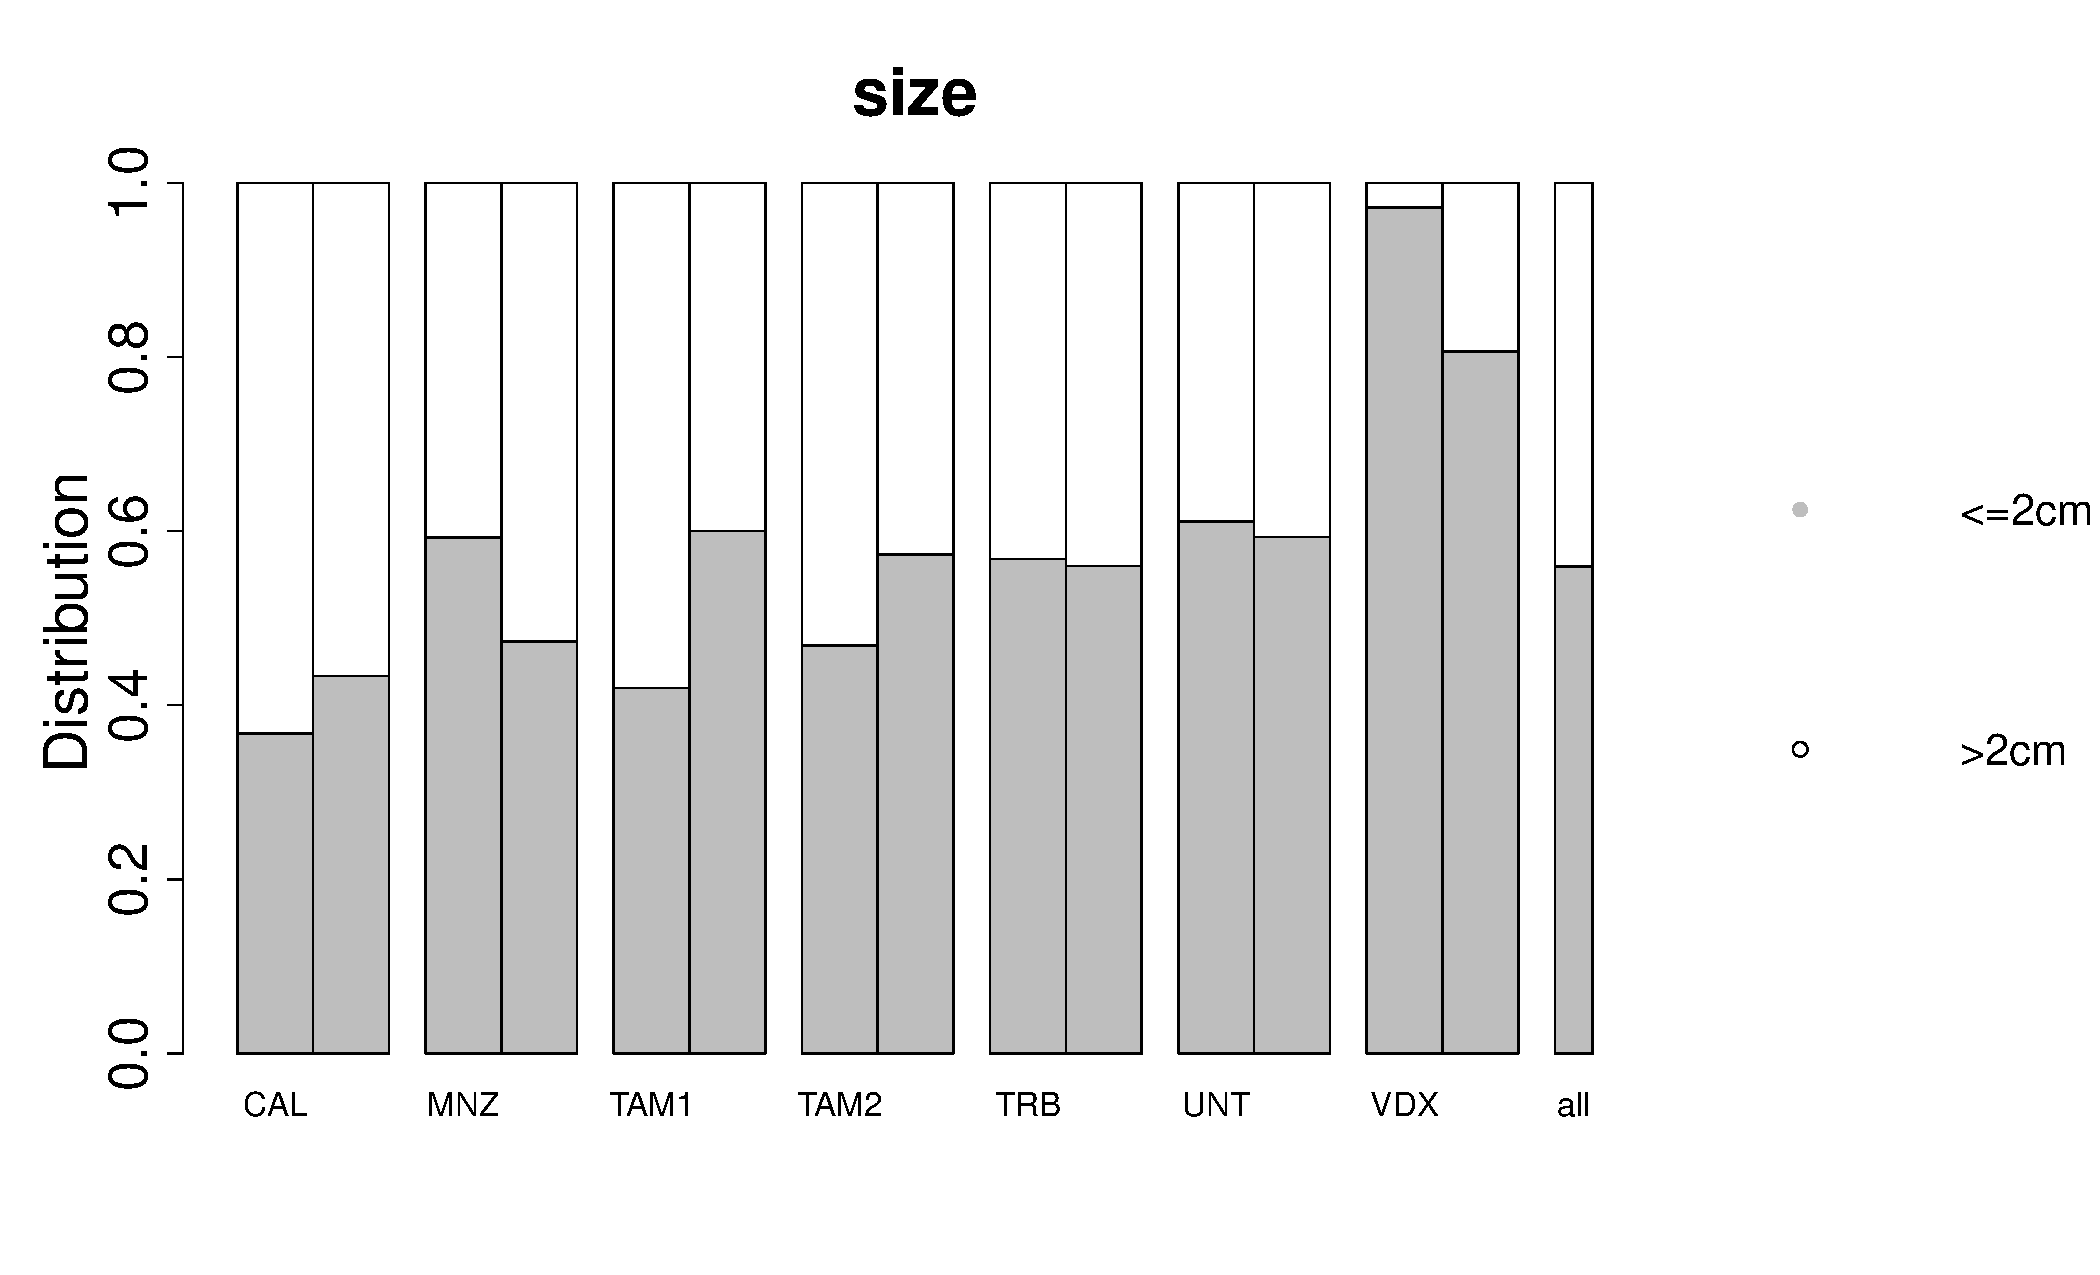
\includegraphics[width=8.5cm]{barplot_size.pdf}
        \end{minipage}
        %\begin{minipage}[b]{0.5\textwidth}
        %    \includegraphics[width=7cm]{node-margin.pdf}
        %\end{minipage}%
        \begin{minipage}[b]{0.5\textwidth}
            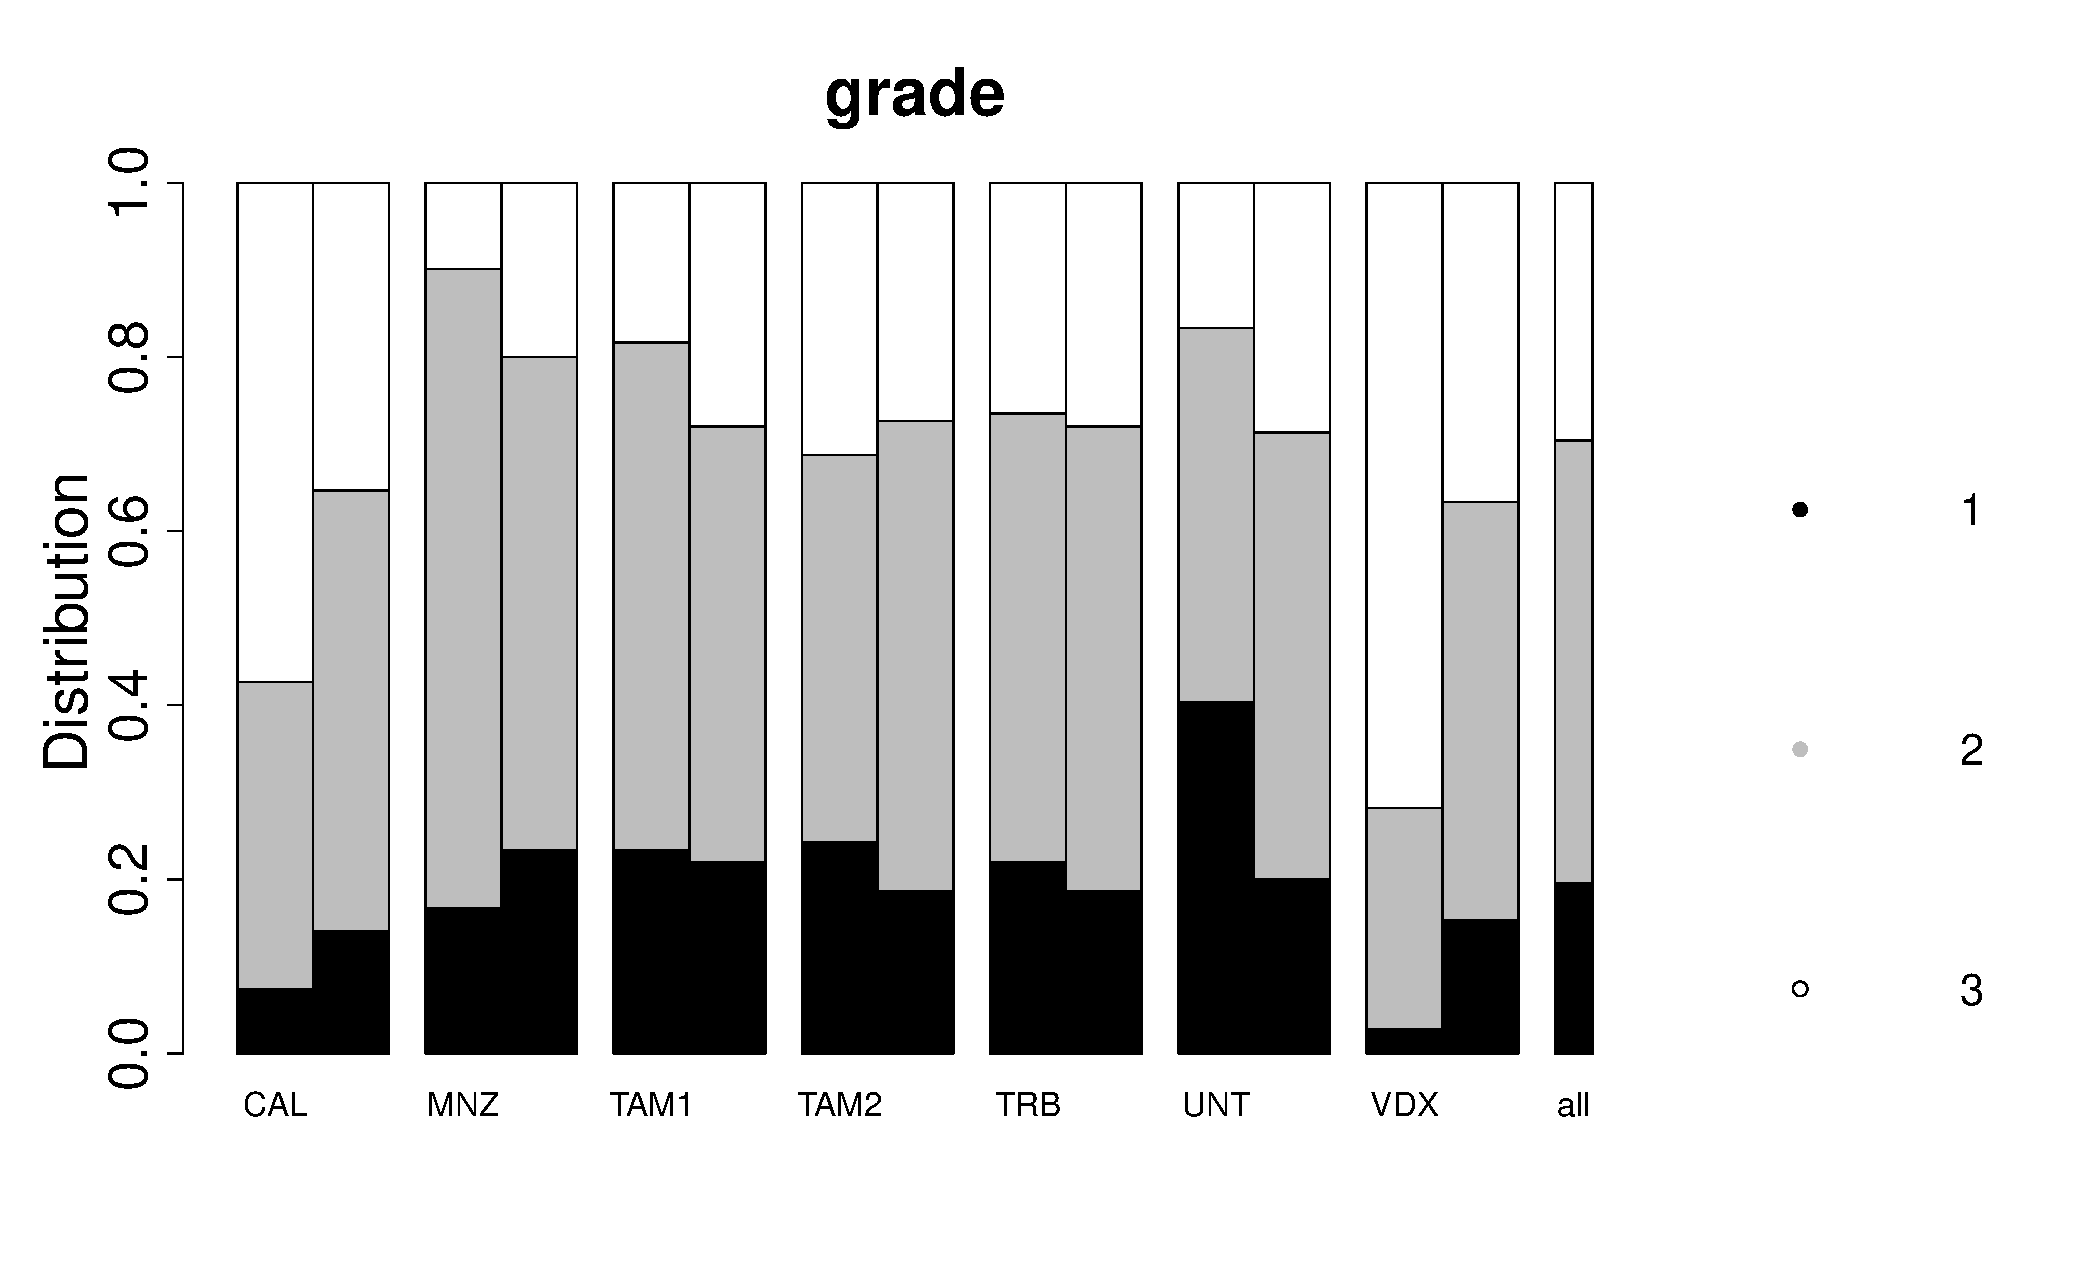
\includegraphics[width=8.5cm]{barplot_grade.pdf}
        \end{minipage}
    \label{barplots}
  \end{figure}

\begin{figure}[H]
\centerline{Ovarian Cancer}
      \centering
        \begin{minipage}[b]{0.5\textwidth}
            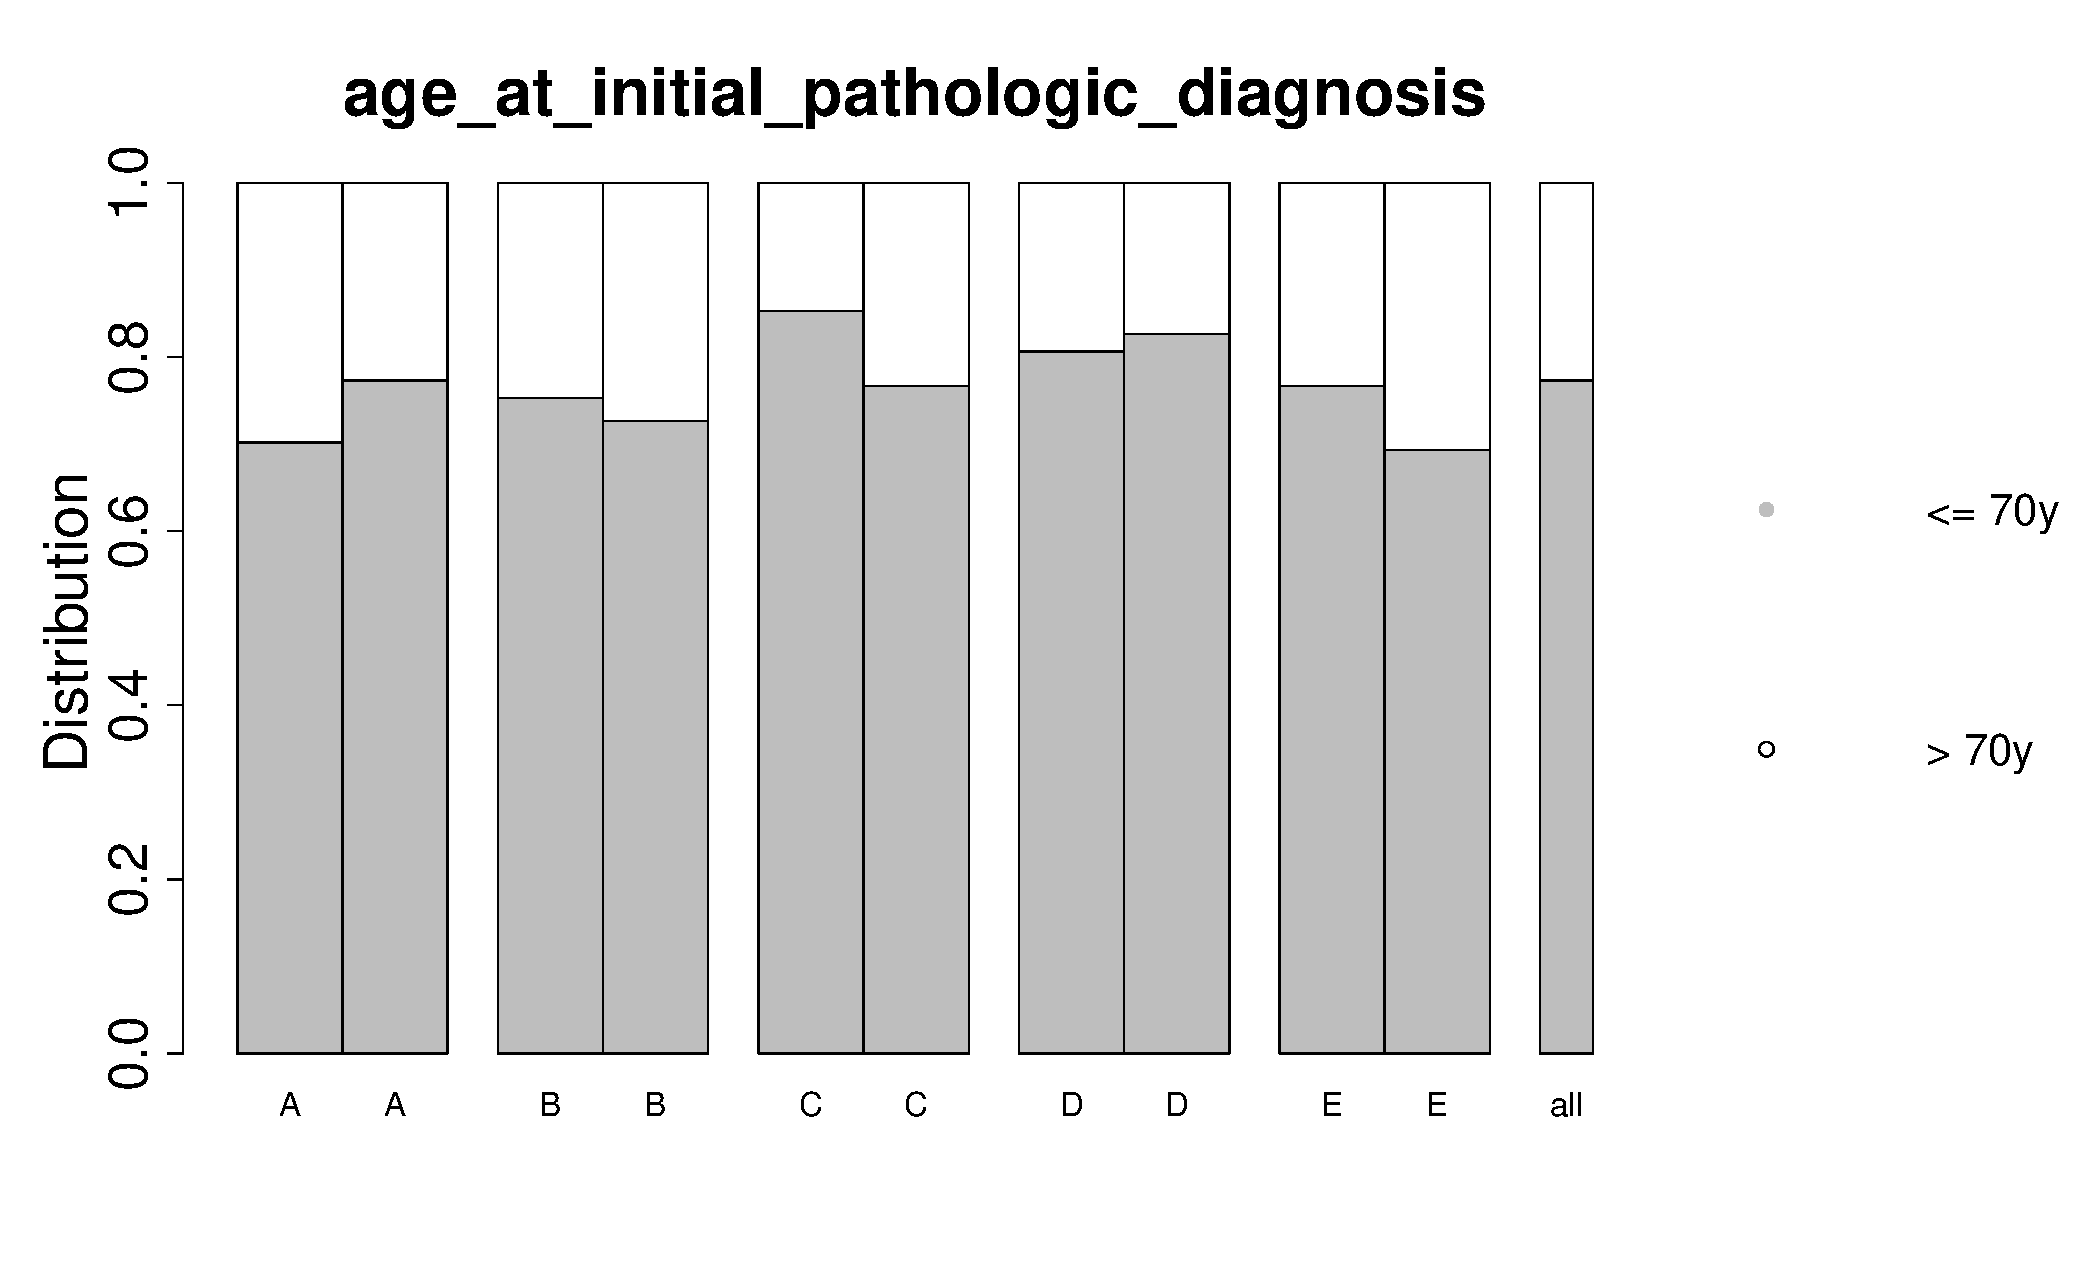
\includegraphics[width=8.5cm]{barplot_ovarian_age.pdf}
        \end{minipage}%
        \begin{minipage}[b]{0.5\textwidth}
            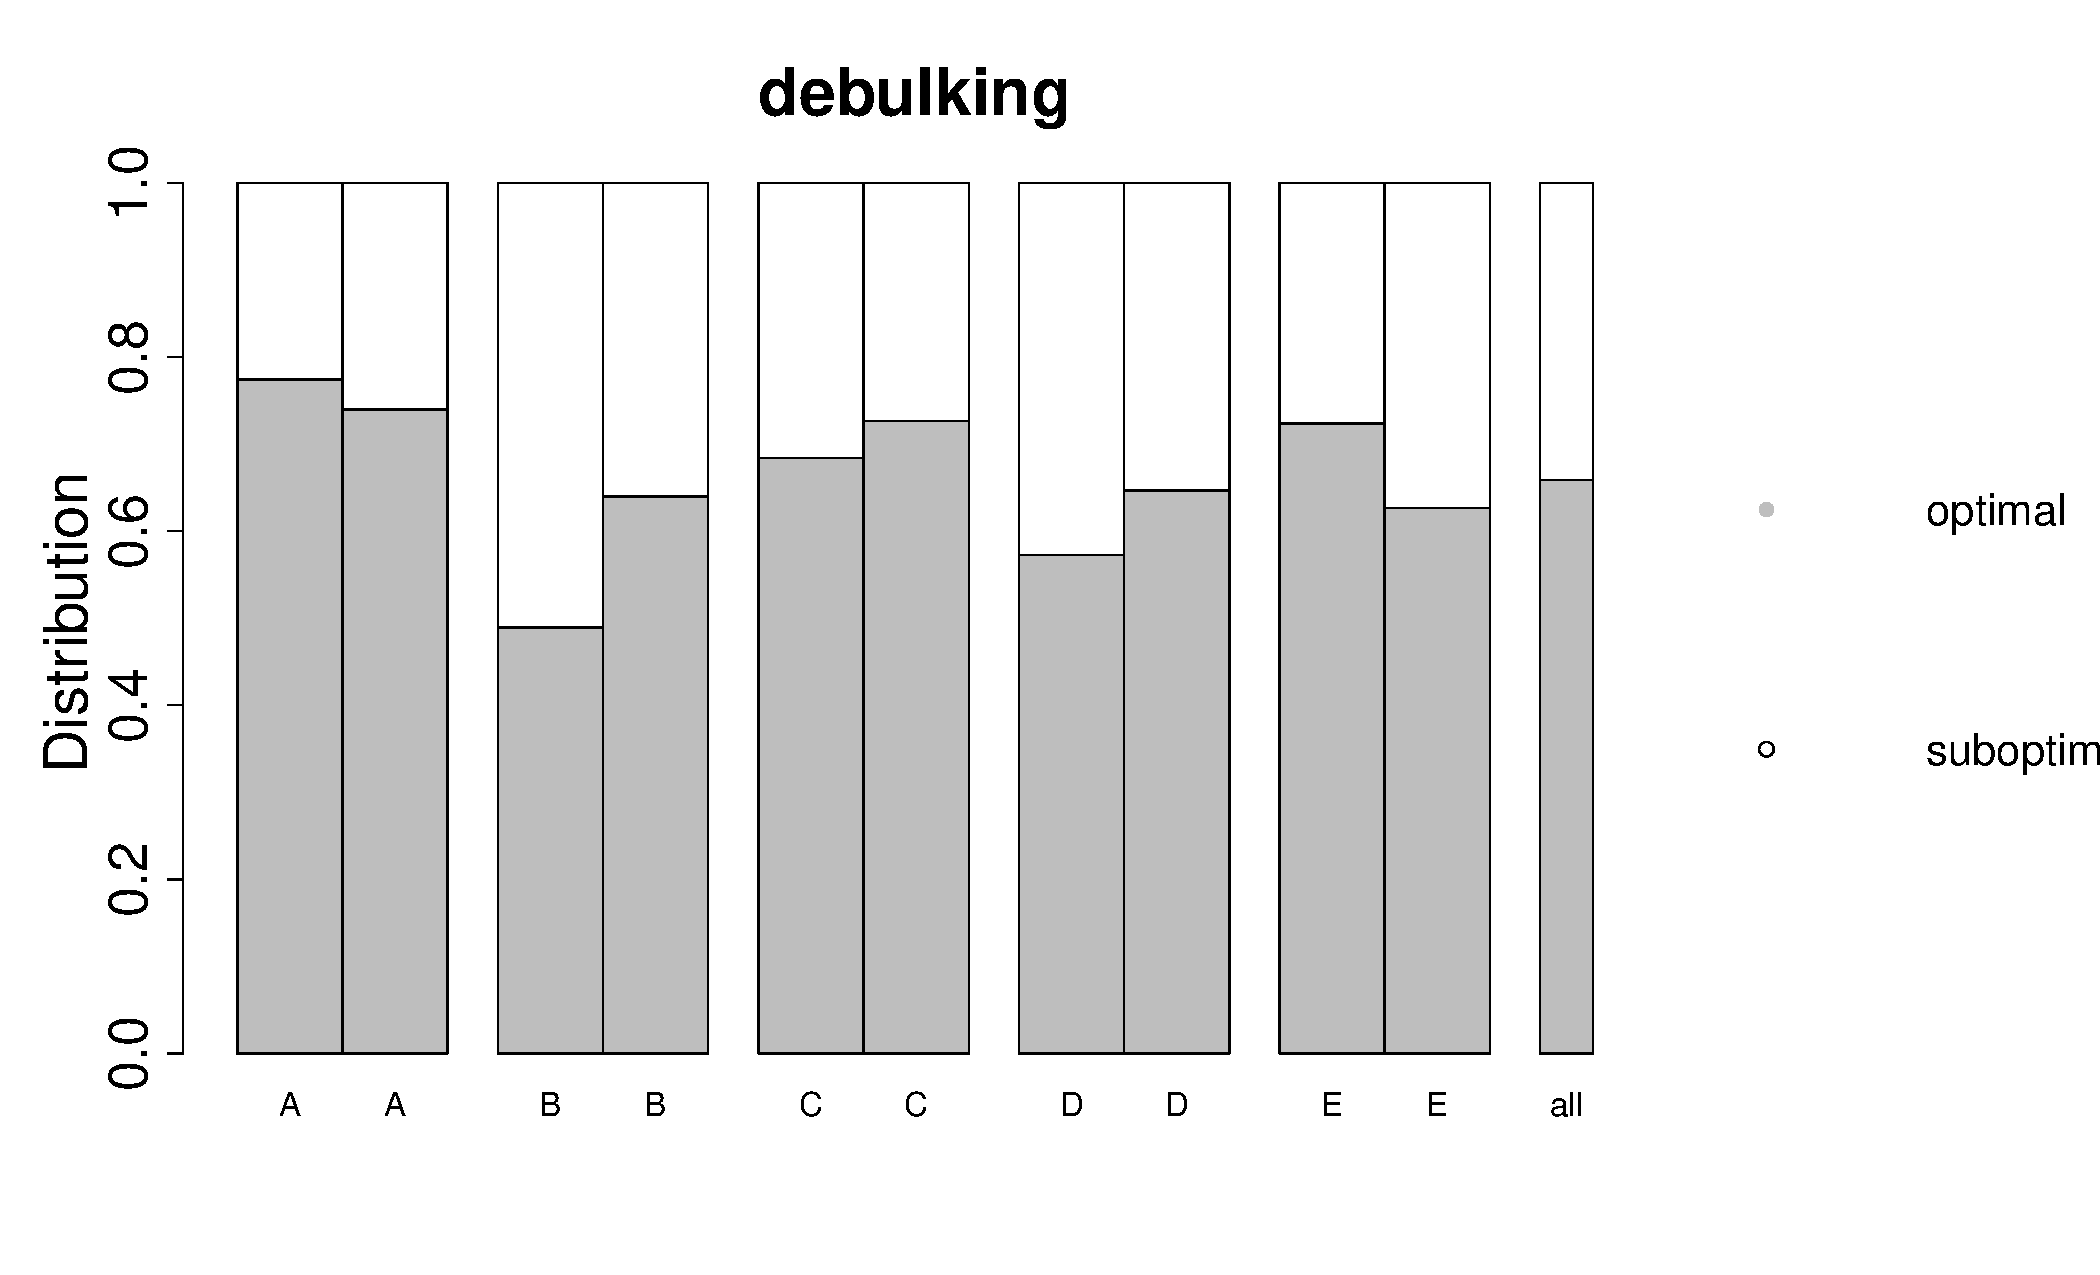
\includegraphics[width=8.5cm]{barplot_ovarian_debulk.pdf}
        \end{minipage}
%        \begin{minipage}[b]{0.5\textwidth}
%            \includegraphics[width=7cm]{barplotsOvarian-barplot-3.pdf}
%        \end{minipage}%
%        \begin{minipage}[b]{0.5\textwidth}
%            \includegraphics[width=7cm]{barplotsOvarian-barplot-4.pdf}
%        \end{minipage}
    \caption{Comparison before and after balancing covariates. It is to illustrate the balancing effect after we adjust the probability of re-sampling. The single bar on the most right shows the overall distribution of the covariate across all original data sets, which we expect to be the distribution of this covariate in each simulated set after balancing. From left to right, every two close together bars represent the distribution in one data set before(the left bar) and after(the right bar) balancing. Changing the probability will not make the proportion of levels after balancing equal to the overall distribution, so the bars are not exactly the same. But we can observe that the distributions after balancing are closer to the overall distribution than those without balancing. Severe bias is adjusted such as tumor size in VDX and age in TRANSBIG. The figures prove that we actually balanced the prevalence of covariates as we wanted. As a back up to the simulation, it enhances our conclusion about the irrelevance of covariate distributions to C-index performances.}
   \label{barplots-ovarian}
\end{figure}


\newpage
\section{Spaghetti Plots}
\begin{figure}[H]
      \centering
        \begin{minipage}[b]{0.5\textwidth}
            \includegraphics[width=8.5cm]{breast_masomenos_CSV.pdf}
        \end{minipage}%
        \begin{minipage}[b]{0.5\textwidth}
            \includegraphics[width=8.5cm]{breast_masomenos_CV.pdf}
        \end{minipage}
        \begin{minipage}[b]{0.5\textwidth}
            \includegraphics[width=8.5cm]{breast_ridge_CSV.pdf}
        \end{minipage}%
        \begin{minipage}[b]{0.5\textwidth}
            \includegraphics[width=8.5cm]{breast_ridge_CV.pdf}
        \end{minipage}
        \begin{minipage}[b]{0.5\textwidth}
            \includegraphics[width=8.5cm]{ovarian_masomenos_CSV.pdf}
        \end{minipage}%
        \begin{minipage}[b]{0.5\textwidth}
            \includegraphics[width=8.5cm]{ovarian_masomenos_CV.pdf}
        \end{minipage}
    \caption{Spaghetti plots of averaged C-indices in cross-study validation and cross-validation. For each set of simulations where a specific source of heterogeneity is equalized, we took the 100 matrices of C index and computed the average values on every position in the matrix. Each line represents the C indices on a certain position (diagonal for CV, off-diagonal for CSV) in the matrix, which changes along with the simulations regarding different sources. The six sets of simulations on the x-axis correspond to the panels in Figure \ref{boxplots}. 1: baseline simulation, 2: eliminating heterogeneity in clinical covariates, 3: filtering genes with high Integrative Correlation, 4: enforcing identical true models, 5: Using only identical baseline hazards but different coefficients. 6: altering all factors together. The order of CSV scores is shuffled from panel 1 where no source is changed, to panel 2 where the covariates are balanced, especially for the breast cancer / M\'{a}s-o-menos combination. }
    \label{spaghetti}
  \end{figure}


\newpage

\section{Fixed threshold for filtering genes with Integrative Correlation}

  \begin{figure}[H]
      \centering
        \begin{minipage}[b]{1\textwidth}
       		\centerline{Breast Cancer / M\'{a}s-o-menos}
            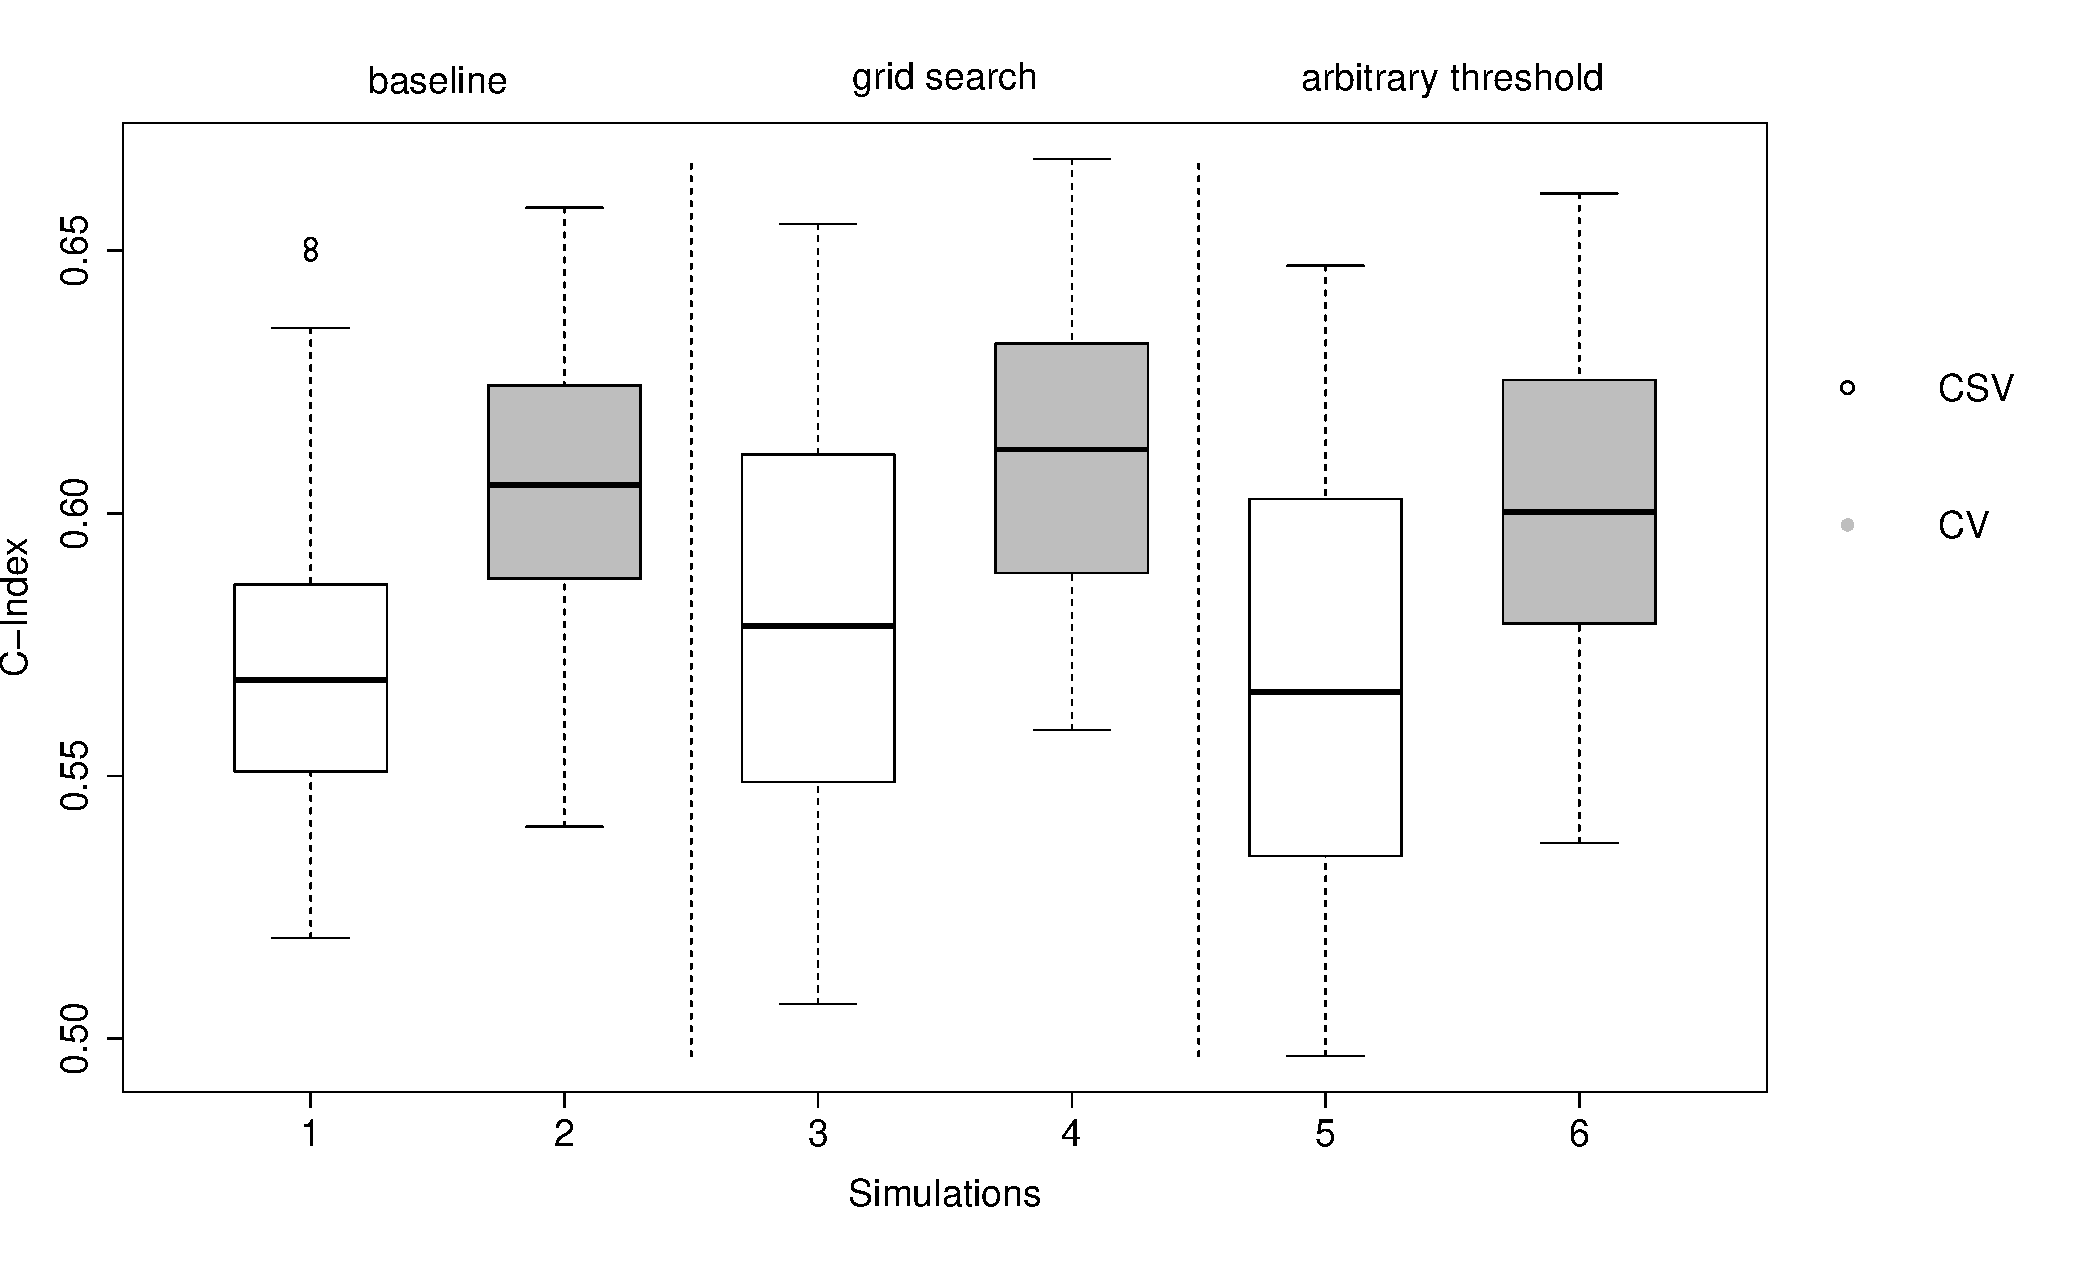
\includegraphics[width=16cm]{breast_masomenos_filter_cutoff.pdf}            
        \end{minipage}
        \begin{minipage}[b]{1\textwidth}
       		\centerline{Breast Cancer / Ridge Regression}
            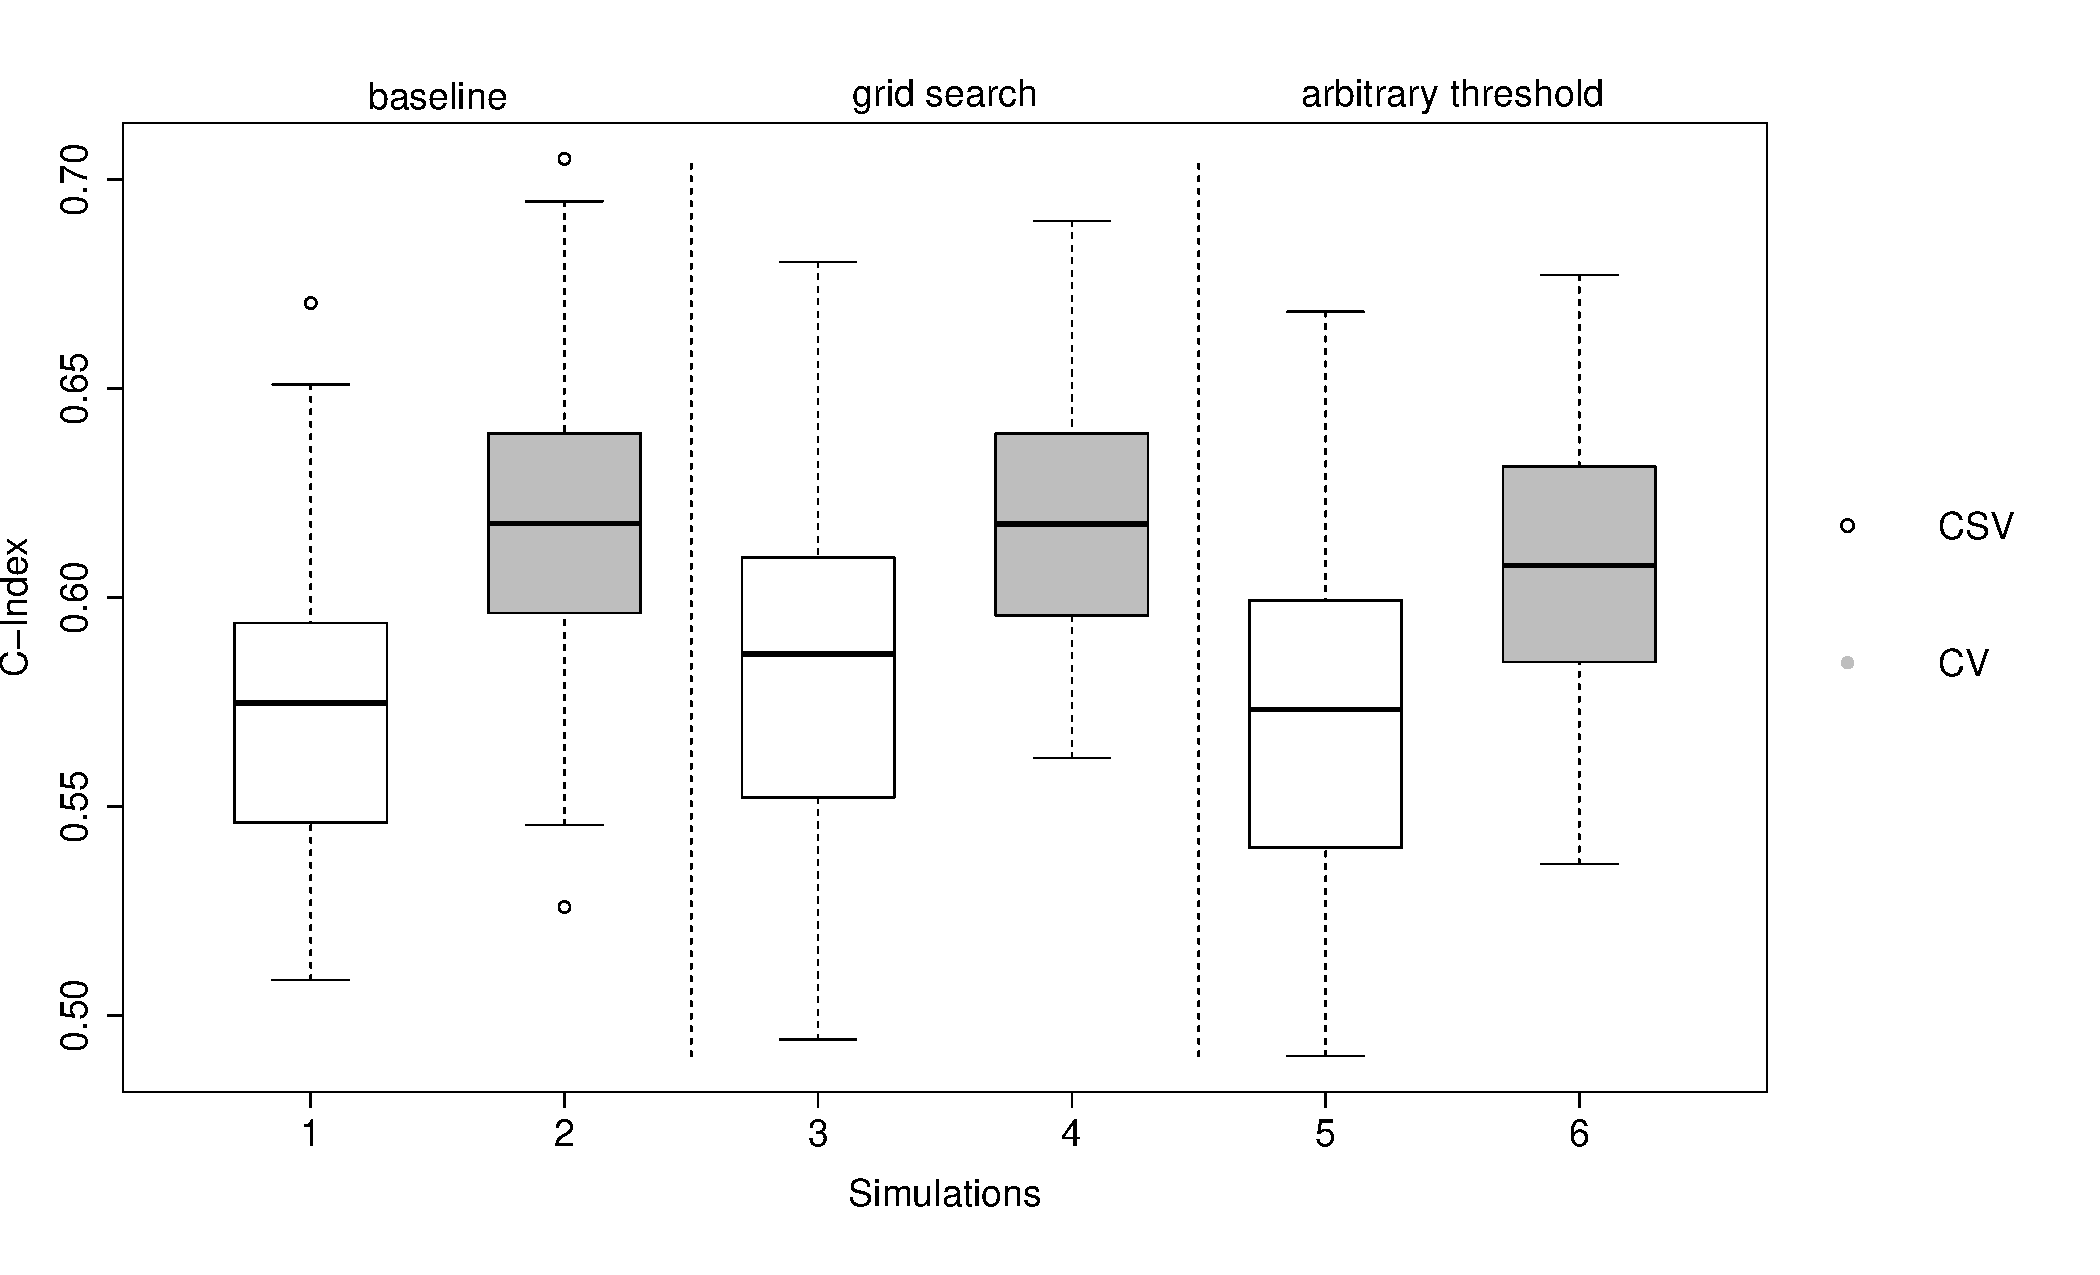
\includegraphics[width=16cm]{breast_ridge_filter_cutoff.pdf}            
        \end{minipage}
  \end{figure}
  \begin{figure}[H]
        	\centerline{Ovarian Cancer / M\'{a}s-o-menos}
            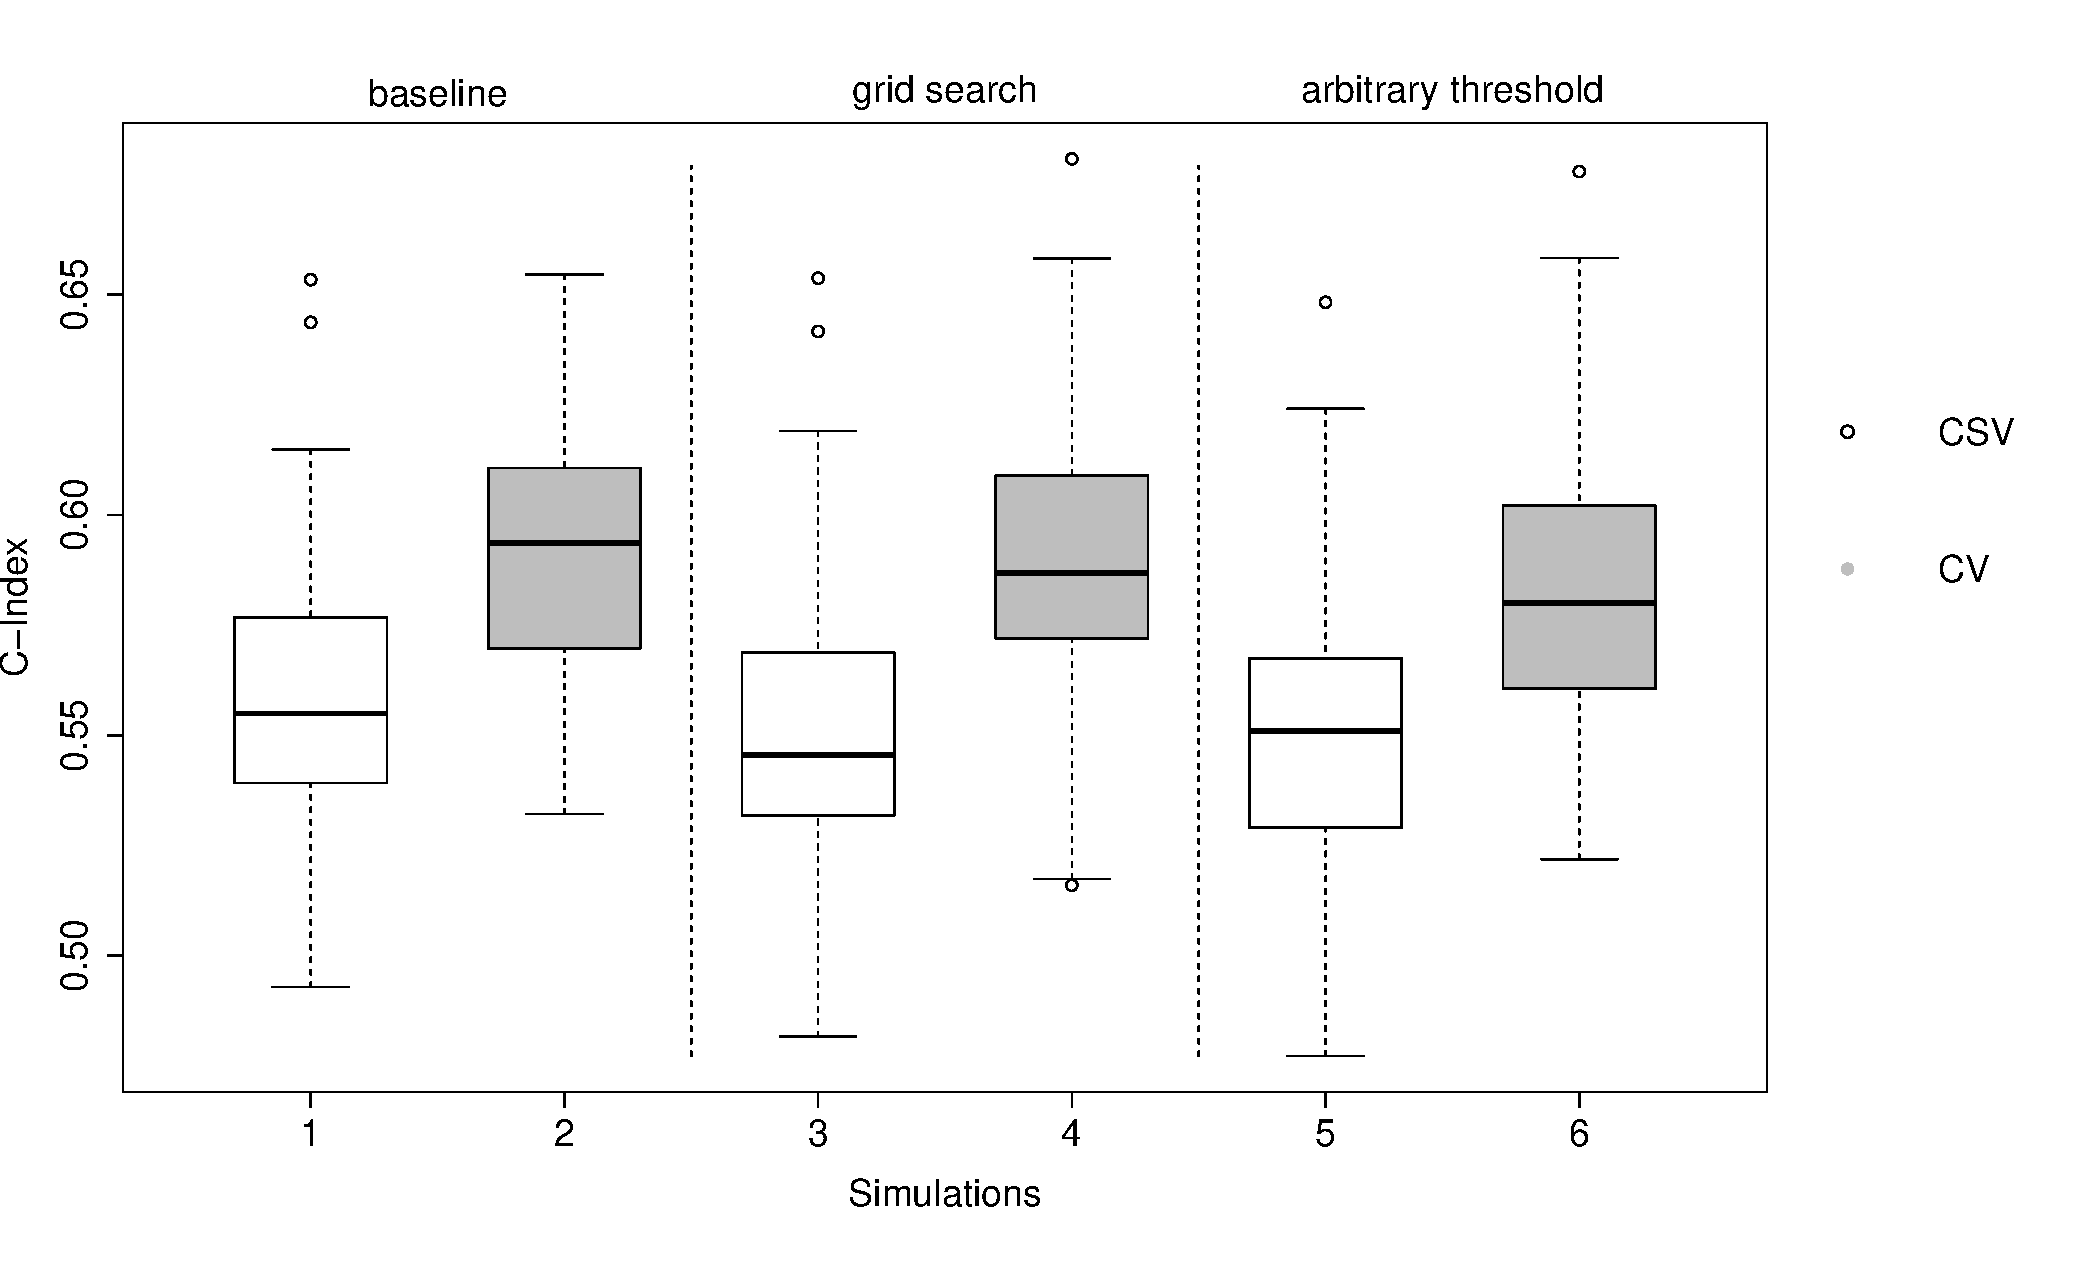
\includegraphics[width=16cm]{ovarian_masomenos_filter_cutoff.pdf}
    \label{filter-cutoff}
    \caption{Boxplots comparing the impact of different thresholds of Integrative Correlation on the simulation result. Baseline: simulation where no sources of heterogeneity are altered, which corresponds to panel "baseline" in Figure \ref{boxplots}. Grid search: we searched on grid for the threshold such that the top 1000 genes with high Integrative Correlations are selected. Arbitrary threshold: the cutoff values of 0.4 for breast cancer and 0.2 for ovarian cancer are used, which includes 343 out of 5307 genes for breast cancer datasets, and 590 out of 7484 genes for ovarian cancer datasets. Both CV and CSV scores generated by using fixed thresholds tend to be worse than baseline, while using the top 1000 genes tends to give better result. The difference between CV and CSV is not reduced with either approach.}
  \end{figure}

%\section{PGR analysis}
%\begin{figure}[H]
%  \centering
%  \includegraphics[width=12cm]{pgranalysis-pgr.pdf}\\
%  \caption{Balancing PGR in the breast cancer / M\'{a}s-o-menos combination. With the five data sets available for pgr, we performed the same cleaning step and conducted the same simulation and validation  procedure. Same as the previous results, the proportion of PGR does not impact the performance of CV or CSV.}
%  \label{pgr}
%\end{figure}

\newpage
\section{Remove CAL}
  \begin{figure}[H]
    \centering
    \begin{minipage}[b]{0.5\linewidth}
    \centerline{(a) Include CAL}
    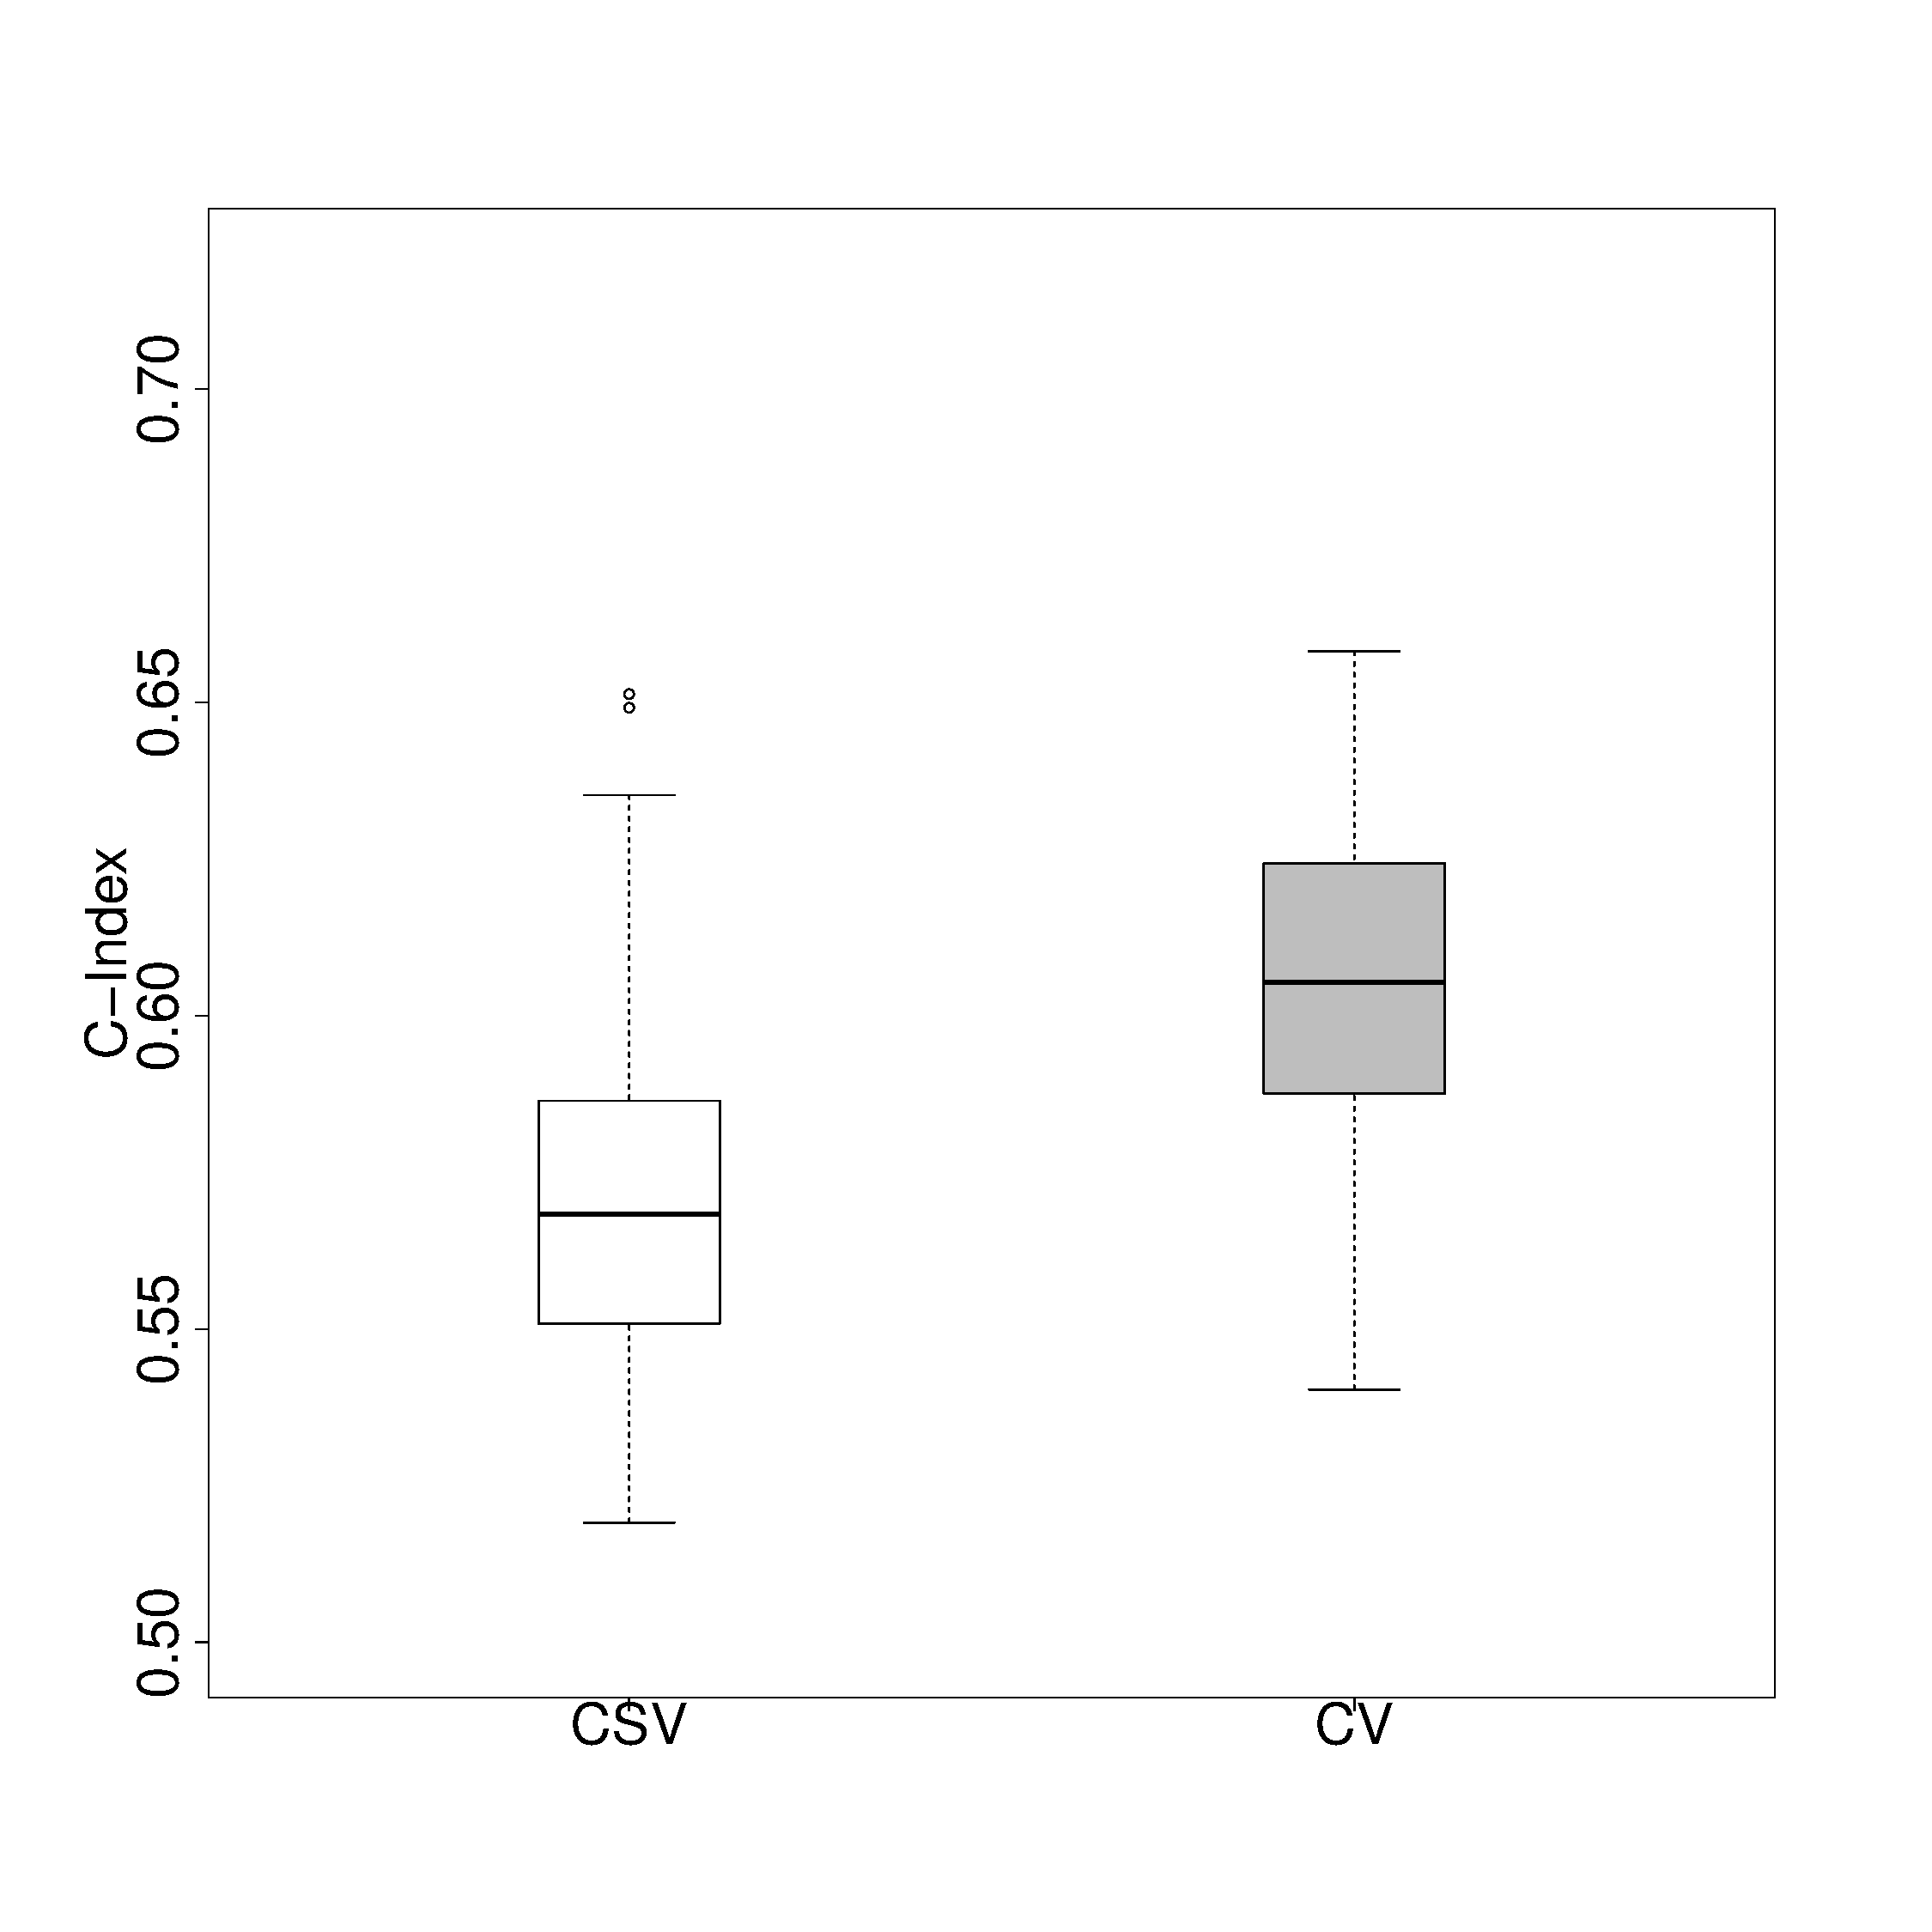
\includegraphics[width=7cm]{boxplot_withCAL.pdf}
    \end{minipage}%
    \begin{minipage}[b]{0.5\linewidth}
    \centerline{(b) Remove CAL}
    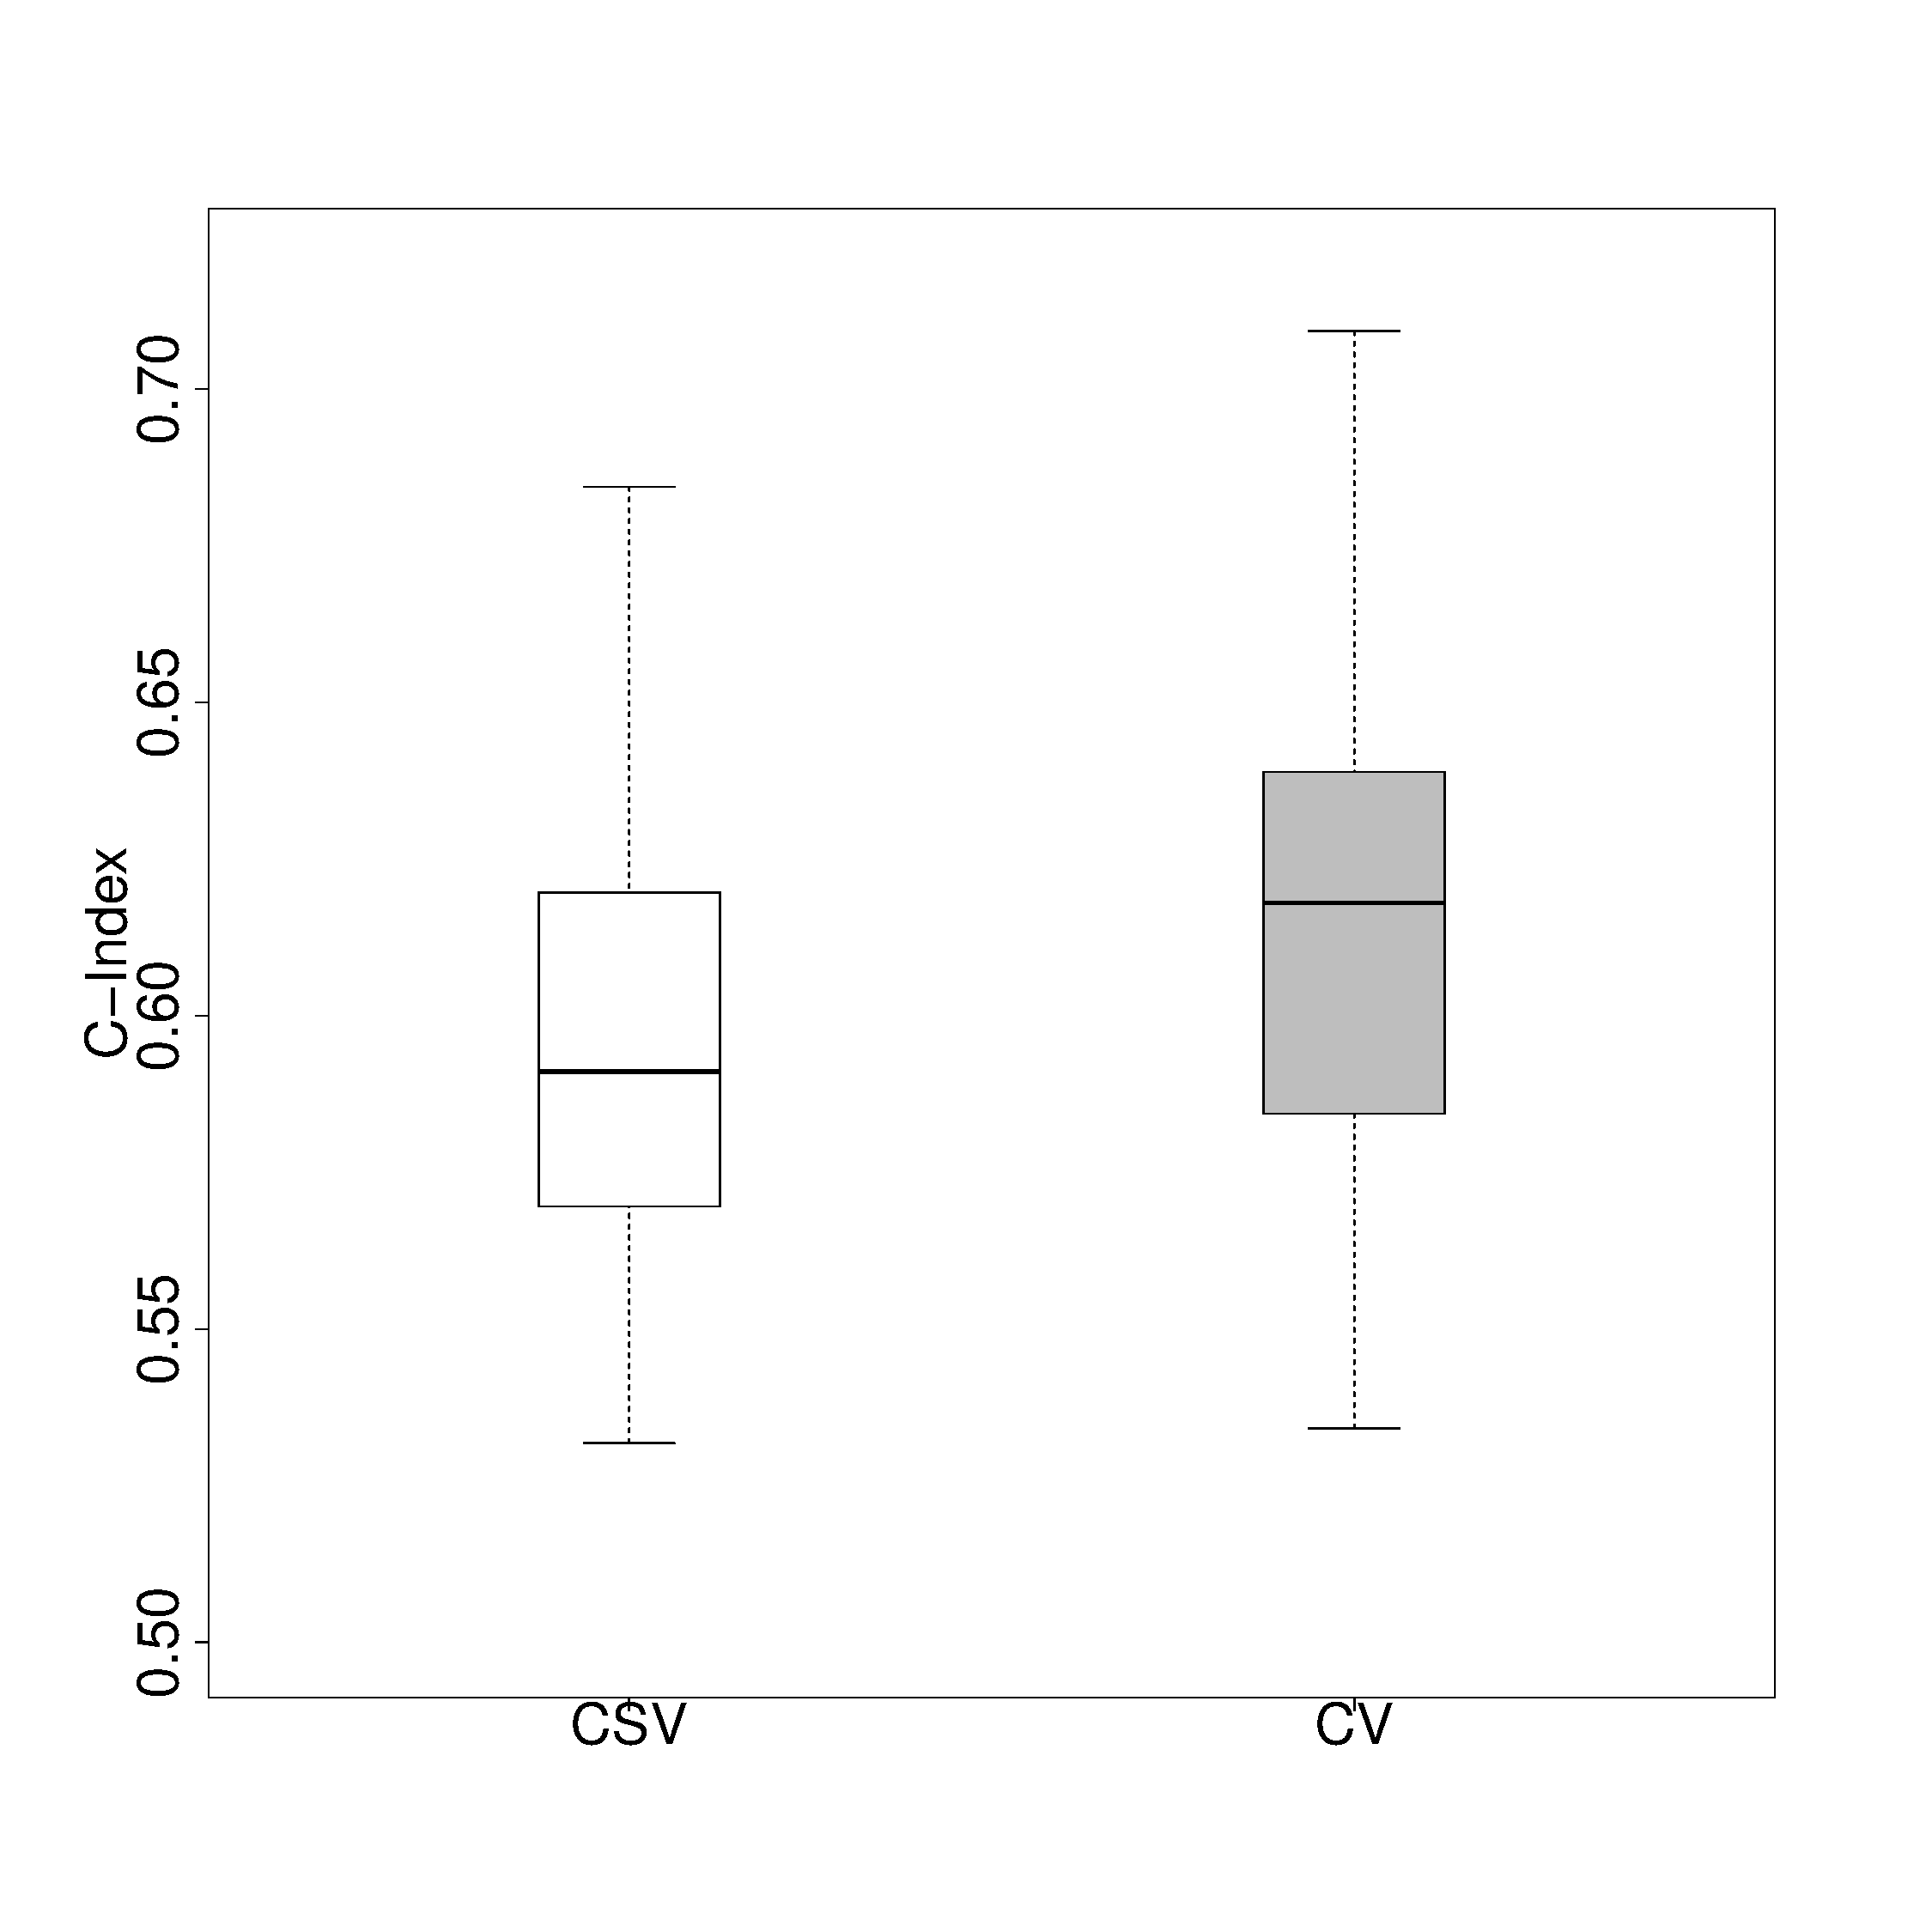
\includegraphics[width=7cm]{boxplot_rmCAL.pdf}
    \end{minipage}
    \caption{Comparison before and after removing CAL under the baseline condition. No factors are considered in this plot. The reduction of difference in C-index between CSV and CV is quite noticeable after eliminating CAL, thus motivates us to repeat the whole simulation without CAL to check if there is any difference in the result. This will be shown in Figure ~\ref{boxplots-outlier}.}
    \label{ourlier-cmp}
  \end{figure}

  %\begin{figure}[H]
  %    \centering
  %      \begin{minipage}[b]{0.5\textwidth}
  %      \centerline{(a) Balance covariates}
  %          \includegraphics[width=7cm]{removeoutlierset-covariates-boxplots-balancing-covariates.pdf}
  %      \end{minipage}%
  %      \begin{minipage}[b]{0.5\textwidth}
  %      \centerline{(b) Filter genes with Integrative Correlation}
  %          \includegraphics[width=7cm]{removeoutlierset-filtergenes-type2-boxplots-expression-cov.pdf}
  %      \end{minipage}
  %      \begin{minipage}[b]{0.5\textwidth}
  %      \centerline{(c) Use the same true model}
  %          \includegraphics[width=7cm]{removeoutlierset-truemodel-boxplots-same-model.pdf}
  %      \end{minipage}%
  %      \begin{minipage}[b]{0.5\textwidth}
  %      \centerline{(d) Combination of different sources}
  %          \includegraphics[width=7cm]{alltogether-removeoutlier-boxplots-same-model.pdf}
  %      \end{minipage}
  %  \caption{Simulation Results with CAL removed. Though the absolute gap between CSV and CV diminishes in every plot, the overall tendency under each scenario remains unchanged: Covariate distribution does not make any difference on C-indices; filtering genes with Integrative Correlation improves both performances but does not neutralize the gap between them; the same true model will explain the difference entirely. The simulations eliminating CAL not only rule out the impact of outlier data set on results, but also can be treated as a replication of simulation to show that our observation can be reproduced.}
  %  \label{boxplots-outlier}
  %\end{figure}
  
  \begin{figure}[H]
  	\centering
  	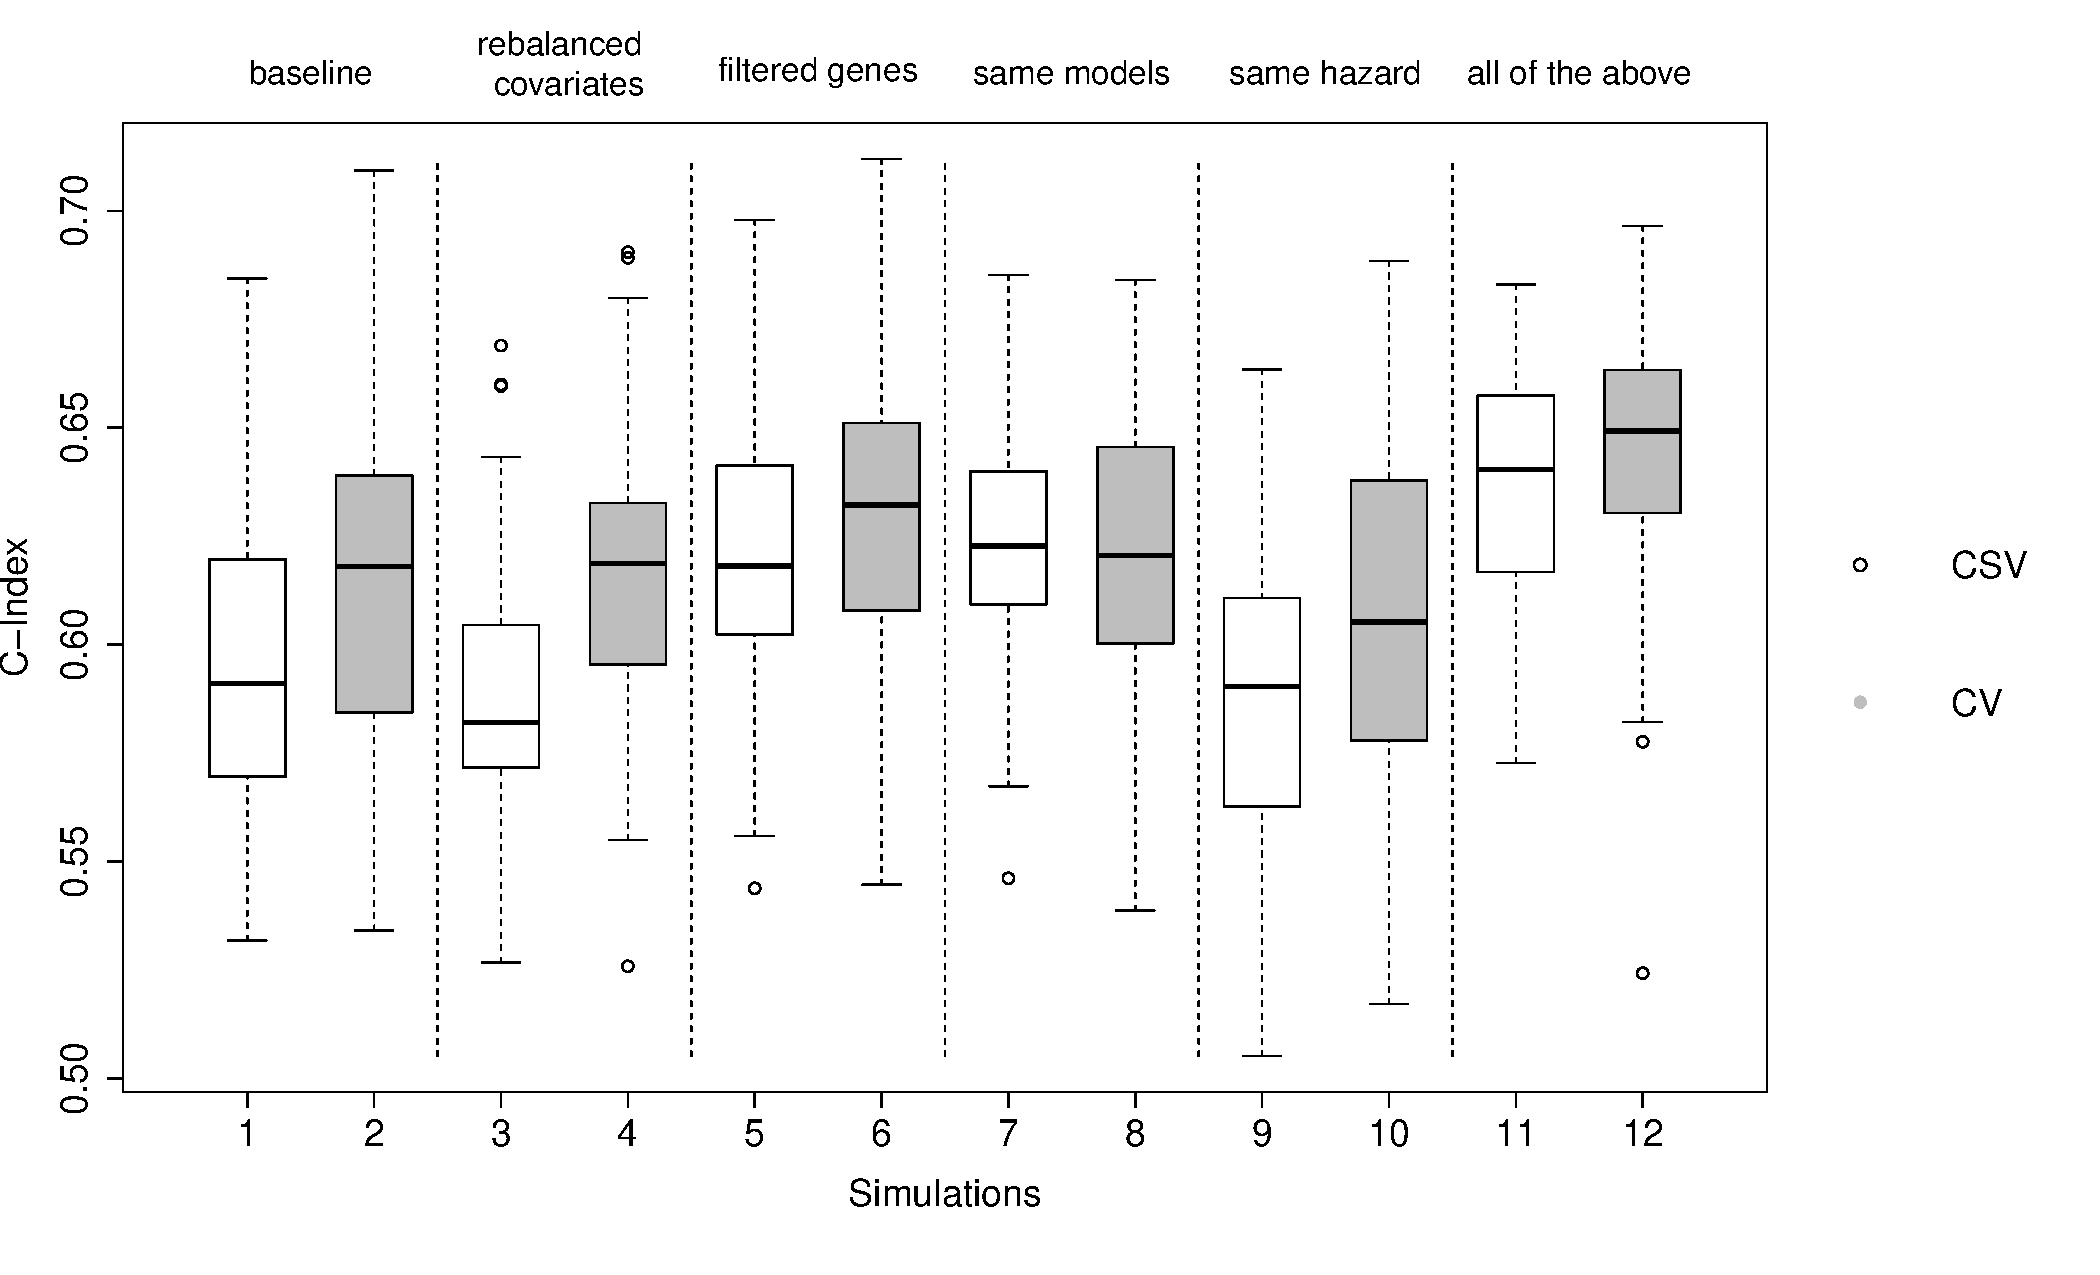
\includegraphics[width=14cm]{rmCAL_boxplot_breast_masomenos_withnames.pdf}\\
  	\caption{Simulation Results with CAL removed. Removing CAL improves both CV and CSV, and it affects CSV more than CV. The absolute value of the CV-CSV difference is reduced in almost every simulation. However, compared to Figure \ref{boxplots}, the results stay robust after the outlier data set is removed, which rules out its influence on the conclusions.}
  	\label{boxplots-outlier}
  \end{figure}
  

\end{document}
